% !TeX root = main.tex
\documentclass[letterpaper, 12pt, oneside]{article}

\usepackage[utf8]{inputenc} %Para configuración de caracteres
\usepackage[spanish]{babel} %Para configuración de idioma

\usepackage{float} %Para que funcionen las tablas
\usepackage{anysize} %Para usar márgenes
\marginsize{3cm}{2.5cm}{1cm}{2cm} %{izquierda}{derecha}{arriba}{abajo}. La superior esta sobre 1, la derecha sobre -0.5 y la de abajo sobre 2 (por el número de página)

%tablas
\usepackage{booktabs}
\usepackage{longtable}
%rotar tablas (y usar \includegraphics )
\usepackage{rotating}
%Dividir en diagonal
%\usepackage{slashbox}
%color tablas
\usepackage{colortbl}
%colocar tabla en lugar de cuadro

\usepackage[numbib,notlof,notlot,nottoc]{tocbibind} %Para que la biliografía se llame así y no referencias y para que quede numerada como sección.
%\usepackage[notlof,notlot,nottoc]{tocbibind} %Bibliografía sin numerar
\bibliographystyle{ieeetr} %Estilo de bibliografía IEEE

\usepackage{url} % inserción url's notas de pie.

%Para poder colocar texto en color
\usepackage{color}
\definecolor{naranja}{rgb}{1,0.5,0} % valores de las componentes roja, verde y azul (RGB)
\definecolor{rojo}{rgb}{1,0,0}
\definecolor{SteelBlue}{rgb}{0.3,0.5,0.7}

%Para tener los bookmarks del pdf (menú al lado derecho en los visualizadores de pdf)
% si colorlinks= true, no salen las cajas, sino el color del link!!
% linkcolor para los indices, citecolor para las citas en texto, urlcolor para los enlaces
\usepackage[pdftex,bookmarks=true, linkcolor=black, citecolor=black, colorlinks=true, urlcolor=black]{hyperref}

%Para poder hacer subfiguras (subfloat)
\usepackage{subfig}

\usepackage{enumitem} % Para poder continuar enumerate en otras partes

\usepackage{pdflscape}%Para colocar páginas horizontales en el PDF

\begin{document}
	
\renewcommand{\tablename}{Tabla}
%%%%%%%%%%%%%%%%%%%%%%%%%%%%%% Portada %%%%%%%%%%%%%%%%%%%%
\newcommand\portada{
\begin{titlepage}
		\begin{center}
			{\bf Diseño e implementación de un launcher Android enfocado a combatir la procrastinación por el uso excesivo del smartphone en estudiantes de pregrado de la Universidad del Valle}
			\vfill
			{\bf Juan Sebastián Ruiz Aguilar}
			\vfill
			{\bf Universidad del Valle\par}
			{\bf Facultad de ingeniería \par}
			{\bf Escuela de ingeniería de sistemas y computación \par}
			{\bf Tuluá, Valle del Cauca \par}
			{\bf 2025 \par}
		\end{center}
\end{titlepage}
}

\newcommand\contraportada{
	\begin{titlepage}
		\begin{center}
			{\bf Diseño e implementación de un launcher Android enfocado a combatir la procrastinación por el uso excesivo del smartphone en estudiantes de pregrado de la Universidad del Valle}
			\vfill
			\vfill
			\vfill
			{\bf Juan Sebastián Ruiz Aguilar \par}
			{\bf Código: 2059898 \par}
			{\url{juan.ruiz.aguilar@correounivalle.edu.co} \par}
			\vfill
			\vfill
			\vfill
			\vfill
			{Director \par}
			{\bf Ing. Héctor Fabio Ocampo Arbeláez \par}
			{Magister en analítica e inteligencia de negocios \par}
			{\url{hector.ocampo@correounivalle.edu.co} \par}
			\vfill
			\vfill
			\vfill
			{\bf Universidad del Valle\par}
			{\bf Facultad de ingeniería \par}
			{\bf Escuela de ingeniería de sistemas y computación \par}
			{\bf Tuluá, Valle del Cauca \par}
			{\bf 2025 \par}
		\end{center}
\end{titlepage}
}

% Ahora llama a los comandos para que se muestren:
\portada
\contraportada

%%%%%%%%%%%%%%%%%%%%%%%%%%%%%% Tabla de contenido %%%%%%%%%%%%%%%%%%%%
\renewcommand\contentsname{\centering Tabla de Contenido}
\tableofcontents

%%%%%%%%%%%%%%%%%%%%%%%%%%%%%% Resumen %%%%%%%%%%%%%%%%%%%%%%%%%%%%%%%
\begin{center}
	\section*{Resumen}	
\end{center}
\addcontentsline{toc}{section}{Resumen} %Añadir resumen a la tabla de contenido

Los estudiantes universitarios que hacen un uso excesivo y/o inadecuado del smartphone tienen un menor rendimiento académico e insatisfacción al no gestionar adecuadamente su tiempo e incumplir los plazos de sus actividades pendientes. Dado que el ecosistema de los teléfonos móviles y sus aplicaciones incentiva a pasar el mayor tiempo posible usándolos, se propone desarrollar una pantalla de inicio (launcher) para teléfonos Android que apunte a reducir la procrastinación mediante una interfaz mínimamente llamativa, a mitigar las distracciones y a gestionar mejor el tiempo invertido dentro de las aplicaciones, principalmente en horarios donde se requiera total disposición a una actividad concreta.

\textbf{Palabras clave:} Procrastinación, Uso Excesivo del Smartphone, Gestión del Tiempo, Launcher Android, Productividad.


%%%%%%%%%%%%%%%%%%%%%%%%%%%%% Introducción %%%%%%%%%%%%%%%%%%%%%%%%%%%%%%%%%
\section*{Introducción.}
\addcontentsline{toc}{section}{Introducción.}
En un mundo conectado digitalmente, donde la tecnología tiene cada vez más alcance y uso en todas las actividades de la vida diaria, es muy común emplear un smartphone para realizarlas o complementarlas. Su amplio abanico de herramientas lo hace apropiado para muchos tipos de tareas y esto hace que, en ocasiones, se emplee gran cantidad de tiempo en ellos, generando distracciones casi inevitables. Esto es perjudicial para las personas que necesitan concentrarse lo mejor posible en su jornada laboral o académica y está afectando, en gran medida, a los estudiantes universitarios.

Los dispositivos móviles y las aplicaciones hoy en día (en especial las empresas detrás de ellos) diseñan sus productos con base en ciertos principios y teorías que fomentan un uso adictivo, teniendo como objetivo retener a los usuarios el mayor tiempo posible dentro de las plataformas \cite{Montag2019} y así maximizar sus ganancias dependiendo del modelo de negocio de cada una. Esto es lo que Santiago Giraldo y Cristina Fernández denominan la \textit{economía de la atención} \cite{Giraldo2020}.

Un estudio realizado a 536 estudiantes de educación superior en Estados Unidos revela que aquellos que pasan una cantidad de tiempo prolongada usando el smartphone ven disminuido su rendimiento académico y su nivel de aprendizaje por las constantes distracciones que genera, además de afectar las variables como la motivación y la autorregulación, aspectos clave en la formación de los individuos \cite{Lepp2015}. Además, muchos de los estudiantes no son conscientes de cuánto tiempo pasan en estos dispositivos: su uso se ha vuelto parte de su rutina desde el primer momento del día y se ven en la necesidad de permanecer conectados \cite{Giraldo2020}. Estos factores propician que la situación se vuelva repetitiva y pueda catalogarse como procrastinación, haciendo que los universitarios acumulen y posterguen sus actividades, trayendo consigo dificultades no solo en las aulas de clase, sino también a nivel personal \cite{Kus2016}, físico \cite{Grewal2020,Puerto2015}, emocional y social \cite{Beutel2016}. 

Para minimizar estos comportamientos y analizar a detalle el uso del smartphone, teniendo en cuenta que aproximadamente el 70\% de los usuarios poseedores de un smartphone a nivel mundial tienen instalado el sistema operativo Android \cite{AndroidUsers2024}, se propone desarrollar un launcher para esta plataforma que ayude a los universitarios a gestionar de mejor manera el tiempo que pasan en su smartphone enfocado a disminuir la procrastinación, especialmente en lo académico, y aumentar sus niveles de productividad y bienestar general.



%%%%%%%%%%%%%%%%%%%%%%%%%%%%% Formulación del problema %%%%%%%%%%%%%%%%%%%%%%%%
\section{Formulaci\'on del problema.}

\subsection{Descripci\'on del problema.}

La forma en la que los estudiantes universitarios llevan a cabo su proceso de formación tiene un gran componente autodidacta que requiere de concentración, autorregulación, autoorganización y autoevaluación tanto en el aula de clase como en otros espacios y tiempos destinados al desarrollo de sus actividades académicas \cite{Rafaila2015}. Su proceso fluye normalmente cuando están presentes varios de estos factores, pero la productividad disminuye al tener distractores constantes en el entorno como pueden ser las notificaciones provenientes del smartphone, un ambiente ruidoso en casa o en espacios fuera del aula de clase. De hecho, el aula de clase también puede convertirse en un espacio propicio a distracciones si la temática de la clase es confusa y/o monótona, conduciendo al uso ineludible del smartphone para desconectar del momento.

Estos dispositivos se convierten en un escape, una salida rápida de los momentos difíciles, la soledad, las responsabilidades, entre otros. Además, se expande hasta abarcar una gran porción de tiempo en la vida diaria, reduciendo o eliminando los momentos que se deberían usar para el crecimiento personal y profesional, subestimando los plazos de entrega de sus pendientes pensando que aún hay tiempo suficiente y que se cuenta con la capacidad de elaborarlos, sin pensar en consecuencias futuras \cite{Lizbeth2023}.

A pesar de que muchos de los estudiantes son conscientes del uso excesivo que hacen de las plataformas móviles \cite{Giraldo2020, Beutel2016}, se crea una bola de nieve de insatisfacción, frustración, estrés y ansiedad por postergar sus actividades, no cumplir sus objetivos, no entregar a tiempo sus trabajos y no interiorizar adecuadamente el conocimiento adquirido, haciendo que el rendimiento en su proceso formativo disminuya y su estabilidad emocional se vea afectada. Todos estos sentimientos solo acentúan más el problema de la procrastinación por el uso del smartphone porque se sigue recurriendo a él buscando dopamina que genera, dando paso a una mala gestión del tiempo y deteriorando la calidad de los resultados esperados en sus actividades.

El uso prolongado de plataformas móviles como redes sociales y servicios de streaming afecta negativamente varios aspectos de la vida de los estudiantes incluyendo el rendimiento académico, la salud mental y el bienestar, el desarrollo social y la adicción a los dispositivos. Las empresas que dirigen este sector utilizan estrategias de diseño psicológico, como el uso del color, el texto y la tipografía, para mantener a los usuarios más tiempo en sus aplicaciones, creando un sentido de urgencia y pertenencia a través de notificaciones constantes y actualizaciones frecuentes de contenido y características nuevas, aprovechándose de aspectos primitivos de la misma psicología humana \cite{Neyman2017}.

Preocupa aún más si se tiene en cuenta que, según estadísticas del Ministerio de Educación de Perú, la mayoría de los estudiantes de educación superior, concretamente el 65\%, se encuentra en el rango entre los 18 y 25 años \cite{UniversidadCifras2023}, mismo rango en el cual se determinó que los universitarios tienen un alto grado de procrastinación y que es significativamente mayor que aquellos por encima de los 25 años \cite{Rodriguez2017}.

Por todos los problemas mencionados surge la necesidad de, a través del mismo dispositivo en el que los estudiantes universitarios reinciden en un comportamiento adictivo, regular el uso de las aplicaciones y ayudar a recuperar la excesiva cantidad de tiempo invertido en el smartphone que le corresponde a actividades de mayor importancia, sobre todo a nivel académico y personal.


\subsection{Definici\'on del problema.}

¿Cómo puede una aplicación móvil diseñada para regular el tiempo de uso del smartphone y optimizar la gestión de las asignaciones ayudar a los estudiantes universitarios a minimizar la procrastinación vinculada al uso excesivo de estas plataformas y a mejorar su concentración, autorregulación y productividad en el ámbito académico y personal?

%%%%%%%%%%%%%%%%%%%%%%%%%%%%%% Marco Referencial %%%%%%%%%%%%%%%%%%%%%%%%%%%%%
\section{Marco referencial.}

\subsection{Marco te\'orico.}

\textbf{Procrastinación.} Es el hábito de posponer tareas o responsabilidades cruciales en favor de actividades más inmediatas o gratificantes, aunque menos relevantes a largo plazo. Esta tendencia puede estar influenciada por una variedad de factores psicológicos y ambientales, como la ansiedad ante el fracaso, la falta de motivación intrínseca para completar las tareas asignadas y la presencia constante de distracciones, entre las cuales destaca el uso excesivo del smartphone. La combinación de estos elementos puede llevar a un ciclo perjudicial de aplazamiento continuo, afectando negativamente tanto el rendimiento académico como el bienestar emocional de los estudiantes \cite{Beutel2016}.

\textbf{Tecnología y adicción.} La creciente adicción a la tecnología, particularmente a los dispositivos móviles y sus aplicaciones, ha captado la atención de investigadores y profesionales en salud mental. Estos dispositivos están diseñados con características específicas destinadas a maximizar la participación del usuario, desde las notificaciones constantes hasta la gamificación de las experiencias de usuario. Estas estrategias pueden desencadenar comportamientos adictivos al generar una gratificación instantánea y dificultar la capacidad de autorregulación del tiempo de uso. Como resultado, los usuarios pueden encontrarse atrapados en un ciclo de consumo compulsivo de contenido digital, lo que puede tener repercusiones negativas en su bienestar psicológico y en su capacidad para concentrarse en actividades importantes, como el estudio académico \cite{Montag2019}.

\textbf{Teoría del diseño centrado en el usuario.} Es una metodología orientada a crear productos y servicios que se adapten de manera óptima a las necesidades, preferencias y habilidades de los usuarios finales. El diseño centrado en el usuario implica iteraciones continuas y pruebas de usabilidad para garantizar que el producto final sea fácil de usar y cumpla con las expectativas de los usuarios. Esto implica la creación de prototipos y la realización de pruebas con estudiantes para evaluar la funcionalidad, la accesibilidad y la eficacia del launcher en la mejora de la gestión del tiempo y la reducción de la procrastinación.

\textbf{Psicología del color.} La Psicología del Color resalta cómo los colores influyen en las emociones y el comportamiento humano. En el diseño del launcher, la elección cuidadosa de colores es crucial, ya que puede impactar la motivación, enfoque y compromiso del usuario con las tareas académicas. Los tonos cálidos como el rojo y el naranja pueden estimular la energía y la acción, fomentando la productividad. Mientras tanto, colores suaves como el azul y el verde pueden crear un ambiente tranquilo, ideal para momentos de concentración y estudio. Mantener consistencia en la paleta de colores y su integración con la interfaz del launcher puede mejorar la experiencia del usuario, aumentando su disposición a utilizar la aplicación de manera efectiva para gestionar su tiempo y combatir la procrastinación.

\textbf{Gestión del tiempo.} Es el proceso de planificar, organizar y controlar cómo se utiliza el tiempo disponible para lograr objetivos específicos, tanto personales como profesionales. Implica identificar las tareas prioritarias, asignarles el tiempo adecuado y utilizar técnicas y herramientas para maximizar la eficiencia y la productividad. El launcher podría ofrecer funciones como recordatorios personalizados para tareas importantes, integración de calendario para una visualización clara de horarios y compromisos, y la capacidad de establecer objetivos académicos con seguimiento de progreso. Estas características permitirían a los estudiantes planificar y organizar sus actividades de manera efectiva, evitando conflictos y garantizando el cumplimiento de plazos, mientras identifican áreas de mejora para optimizar su rendimiento académico \cite{Mengual2012}. 

\textbf{Productividad.} Es la capacidad de producir más resultados con la misma cantidad de recursos, o producir los mismos resultados con menos recursos, en un período de tiempo determinado. Esto es esencial para el éxito tanto académico como personal, implicando la eficiencia en la realización de tareas y la obtención de resultados satisfactorios. En el contexto del launcher, se busca potenciar la productividad de los estudiantes mediante la minimización de distracciones y el logro de objetivos de manera efectiva. Esto se logra a través de funciones que permiten enfocarse en tareas prioritarias y limitar las interrupciones, organizar aplicaciones de manera intuitiva para acceder rápidamente a recursos de estudio, y proporcionar herramientas de seguimiento del tiempo para analizar y mejorar la eficiencia en el uso del dispositivo. 


\subsection{Estado del arte.}

El estudio "Adicción a las Redes Sociales y Procrastinación Académica en estudiantes Universitarios" \cite{Luisa2019} encontró una correlación positiva y significativa entre la adicción a las redes sociales y la procrastinación académica, lo que significa que niveles más altos de adicción a las redes sociales corresponden a niveles más altos de procrastinación académica. El estudio también destaca la prevalencia de ambos problemas entre los estudiantes universitarios de todo el mundo, ya que sólo el 15\% de los estudiantes no muestra ningún nivel de adicción a las redes sociales. Los resultados se basan en una muestra de estudiantes de Lima y son relevantes para comprender el impacto de las redes sociales en el rendimiento académico. Este estudio proporciona evidencia de la relación significativa entre la adicción a las redes sociales y la procrastinación académica en estudiantes universitarios, lo cual es una preocupación creciente en la educación superior. Los hallazgos sugieren que abordar la adicción a las redes sociales puede ser una estrategia eficaz para reducir la procrastinación académica y mejorar los resultados de los estudiantes.

El artículo "La Generación Zombie. El uso excesivo de teléfonos celulares en las aulas universitarias peruanas" \cite{Montenegro2023}. Analiza el uso excesivo de celulares por parte de estudiantes universitarios en las aulas de clase y sus efectos negativos en el aprendizaje y la salud. Se destaca que dos tercios de los estudiantes encuestados reconocen que el uso del celular en el aula afecta negativamente su aprendizaje al distraerlos y alejarlos de prestar atención a las actividades académicas. De igual manera resalta que casi el 70\% de los estudiantes está consciente de que el uso excesivo del celular es nocivo para la salud física y mental, generando adicción, problemas de concentración, afectando la interacción humana, etc. Por último, sugieren que las universidades deberían implementar políticas y estrategias para regular el uso de teléfonos móviles en las aulas, como horarios designados para el uso del teléfono y promover el uso responsable.

Adiba Orzikulova destaca los impactos negativos del uso excesivo de teléfonos inteligentes, particularmente en aplicaciones de redes sociales, en los estudiantes universitarios \cite{Orzikulova2022}. El estudio sugiere que las intervenciones de autoayuda basadas en aplicaciones móviles pueden ser efectivas para prevenir el uso excesivo de teléfonos inteligentes y la adicción a los teléfonos inteligentes, pero se necesita más investigación para comprender los mecanismos subyacentes de la adicción a los teléfonos inteligentes y el impacto de estas intervenciones en el comportamiento de los estudiantes. El estudio también enfatiza la importancia de la autorregulación y sugiere que las barreras físicas pueden ser más efectivas para prevenir la adicción a los teléfonos inteligentes y promover la autorregulación que las intervenciones basadas únicamente en software.


\subsection{Marco conceptual.}

\textbf{Aprendizaje autodirigido.} Es un proceso de aprendizaje en el que el estudiante lleva las riendas de su propio proceso educativo. Implica que el alumno identifica de forma autónoma sus necesidades y objetivos de aprendizaje, busca y selecciona los recursos y estrategias más adecuados, y evalúa por sí mismo sus logros y resultados. Requiere que el estudiante emplee habilidades de autorregulación, como estrategias cognitivas, metacognitivas y de motivación personal, ya sea trabajando de manera independiente o con cierta guía externa. En esencia, el aprendiz toma un papel activo y autorresponsable en la conducción de su aprendizaje \cite{Marquez2014}.

\textbf{Launcher Android.} Un launcher en Android es una aplicación que permite personalizar la interfaz de usuario y la apariencia de la pantalla de inicio de un dispositivo móvil. Funciona como una capa de personalización sobre el sistema operativo Android, permitiendo al usuario modificar la disposición de iconos, widgets, fondos de pantalla y otros elementos visuales en la pantalla de inicio. Los launchers ofrecen opciones de personalización avanzadas, como cambiar el diseño de la pantalla de inicio, agregar efectos de transición, modificar los iconos de las aplicaciones y ajustar la organización de las aplicaciones \cite{Launcher}.

\textbf{Autocontrol.} Capacidad de modular y controlar las propias acciones de una forma apropiada a la edad de la persona. Es considerado uno de los componentes clave de la inteligencia emocional que debe ser reeducado en los estudiantes. El autocontrol implica tener una sensación de control interno sobre el propio cuerpo, conducta y entorno, permitiendo regular los impulsos y actuar de manera intencionada para lograr los objetivos deseados. Se plantea que el desarrollo del autocontrol desde la infancia constituye una facultad fundamental en el ser humano para tener una voluntad sólida y capacidad de autogobernarse \cite{Navarro2003}. 

\textbf{Rendimiento académico.} El rendimiento académico se refiere a la evaluación y medición de los conocimientos y habilidades adquiridos por un estudiante durante su formación académica, ya sea en niveles escolares, terciarios o universitarios. Se considera que un alumno tiene un buen rendimiento académico cuando obtiene calificaciones positivas y aprobatorias en los exámenes y evaluaciones que rinde a lo largo de los ciclos o períodos académicos correspondientes \cite{RendimientoEscolar}.

\textbf{Concentración.} La concentración es el enfoque voluntario de la mente hacia un objetivo específico, tarea o actividad, excluyendo cualquier distracción o interferencia que pueda surgir. Es un proceso psíquico que se lleva a cabo mediante el razonamiento, donde se dirige toda la atención hacia un punto determinado, ya sea una tarea en curso o algo en lo que se está pensando \cite{Concentracion2023}.

\textbf{Frustración.} La frustración es un estado emocional caracterizado por sentimientos de decepción, irritabilidad o insatisfacción que surgen cuando una persona experimenta obstáculos o dificultades para alcanzar sus metas o satisfacer sus necesidades. Se manifiesta como una respuesta emocional negativa frente a la percepción de que los esfuerzos realizados no han dado los resultados deseados. La frustración puede surgir en diversas situaciones de la vida cotidiana, como problemas laborales, académicos, personales o sociales, y puede tener efectos adversos en el bienestar emocional y el comportamiento de la persona afectada \cite{Kamenetzky2009}.

%%%%%%%%%%%%%%%%%%%%%%%%%%%%%% Alcance %%%%%%%%%%%%%%%%%%%%%%%%%%%%%%
\section{Alcance.}	

\subsection{Declaración del alcance.}

El alcance del presente trabajo de grado consiste en el desarrollo de un launcher Android personalizado para estudiantes de la Universidad del Valle en Tuluá que incorpore las siguientes funcionalidades: 

\begin{enumerate}
    \item \textbf{Diseño minimalista:} Contará con una interfaz sin íconos de aplicaciones para evitar desviar la atención, en tonos neutrales y con atajos útiles para gestionar las demás características presentes en el launcher.
    \item \textbf{Seguimiento del tiempo de uso de las aplicaciones:} El tiempo que se pasa en ciertas aplicaciones seleccionadas por el estudiante se podrá regular y monitorear con el fin de registrar progreso o áreas de mejora.
    \item \textbf{Gestión de tareas y hábitos:} El launcher permitirá consignar las tareas que se deseen realizar y crear hábitos en función de tareas, tiempo límite o chequeo regular del hábito en cuestión.
    \item \textbf{Herramienta(s) de productividad:} Se integrará al menos una herramienta de productividad para apoyar la realización de las tareas o los hábitos, como técnicas de distribución del tiempo de sesiones de trabajo, priorización de tareas, entre otras.
\end{enumerate}

%%%%%%%%%%%%%%%%%%%%%%%%%%%%%%%%%%%%%%%%%%%%

\subsection{Supuestos.}

\begin{enumerate}
    \item Correcto funcionamiento de los equipos donde se llevará a cabo el desarrollo y las pruebas del proyecto. 
    \item Normal desarrollo de los periodos académicos.
    \item Continuidad laboral del director de trabajo de grado.
\end{enumerate}

%%%%%%%%%%%%%%%%%%%%%%%%%%%%%%%%%%%%%%%%%%%%

\subsection{Restricciones.}

\begin{enumerate}
    \item El proyecto se debe llevar a cabo en un plazo máximo de ocho (8) meses.
    \item Solo estará disponible para el sistema operativo Android.
    \item Será diseñado para el tamaño y la interfaz de un smartphone, no para tablets u otros dispositivos similares.
    \item El proyecto y anteproyecto deben ser aprobados.
\end{enumerate}



%%%%%%%%%%%%%%%%%%%%%%%%%%%%%% Objetivos %%%%%%%%%%%%%%%%%%%%%%%%%
\section{Objetivos.}

\subsection{Objetivo general.}

Desarrollar un launcher Android personalizado para regular el uso del Smartphone y aumentar la productividad de los estudiantes de la Universidad del Valle en Tuluá.

\subsection{Objetivos espec\'ificos.}	

\begin{enumerate}
    \item Definir los requisitos funcionales de una pantalla de inicio para Android.
    \item Diseñar la arquitectura interna e interfaces gráficas de la aplicación.
    \item Integrar el diseño y las funcionalidades en la aplicación de acuerdo con los requisitos establecidos.
    \item Implementar pruebas unitarias y de usabilidad del launcher en un sistema Android.
\end{enumerate}

\subsection{Resultados esperados.}	

\begin{table}[H]
\caption{Resultados esperados}
\begin{tabular*}{\textwidth}{|p{0.5\textwidth}|p{0.5\textwidth}|}
\cline{1-2}
\multicolumn{1}{|c|}{\cellcolor[gray]{0.9} \textbf{Objetivo específico}} &  \multicolumn{1}{|c|}{\cellcolor[gray]{0.9} \textbf{Resultados esperados}}  \\
\cline{1-2}
1. Definir los requisitos funcionales de una pantalla de inicio para Android. & 
Documento donde se describan las secciones y herramientas que incorporará, lenguajes y tecnologías a emplear.
\\
\cline{1-2} 

2. Diseñar la arquitectura interna e interfaces gráficas de la aplicación. & 
Diseño de las vistas de la aplicación con sus elementos e interacciones como un prototipo; especificación de la arquitectura que se usará para la estructuración del código y los componentes del launcher.
\\

\cline{1-2} 

3. Integrar el diseño y las funcionalidades en la aplicación de acuerdo con los requisitos establecidos. & 
Código fuente del launcher con el diseño y las características definidas con anterioridad. \\

\cline{1-2} 

4. Implementar pruebas unitarias y de usabilidad del launcher en un sistema Android. & 
Informe de las pruebas a nivel de código y de experiencia de usuario del launcher instalado en un dispositivo Android. \\

\cline{1-2} 

\end{tabular*}
\end{table}







%%%%%%%%%%%%%%%%%%%%%%%%%%%%%% Metodología %%%%%%%%%%%%%%%%%%%%%%%%%
% \pagebreak
% \section{Metodología.}

\section{Metodología.}

\subsection{Tecnologías empleadas.}

En el panorama actual del desarrollo móvil, los desarrolladores se enfrentan a una decisión fundamental entre el desarrollo nativo y multiplataforma. Con el crecimiento exponencial del mercado de aplicaciones móviles y la demanda de experiencias de usuario cada vez más sofisticadas, la elección tecnológica se convierte en un factor determinante para el adecuado desarrollo del proyecto. Así pues, se realizó una evaluación de las tecnologías disponibles, considerando las necesidades específicas y las tendencias actuales de la industria.

\subsubsection{Versión objetivo de la API de Android.}

La elección de Android 10 (API 29) como versión mínima para el desarrollo de Dino Launcher se fundamenta en la convergencia entre las funcionalidades que introduce esta versión del sistema operativo, los requisitos específicos del launcher desarrollado y la posibilidad de que pueda ser ejecutado en dispositivos no tan recientes de manera satisfactoria. En la figura \ref{fig:versiones_android}, los datos de distribución de Android 10 alcanzan el 81.2\% de los dispositivos en el mercado, lo que garantiza una amplia compatibilidad con los dispositivos de los usuarios objetivo. 

\begin{figure}[H]
\caption{Distribución de versiones de Android a nivel mundial. \cite{AndroidStudio}}
\label{fig:versiones_android}
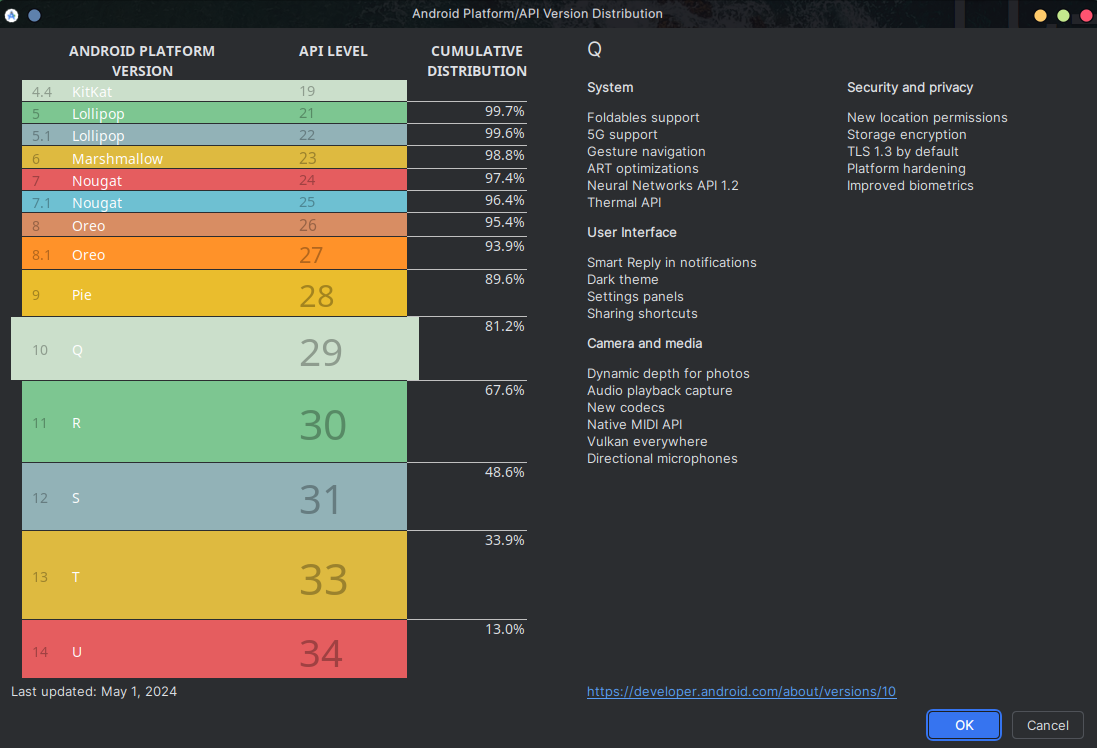
\includegraphics[width=\textwidth]{Figuras/versiones_android.png}
\centering
\end{figure}

Esta versión introduce características esenciales que hacen posible una de las funcionalidades centrales del launcher, la introducción nativa del \textbf{modo oscuro}. Esta permite al launcher mostrar automáticamente los modos claro y oscuro dependiendo de la configuración del tema del sistema, reduciendo significativamente la fatiga visual durante el uso del launcher y mejorando la experiencia de usuario, especialmente durante las horas nocturnas cuando el control del tiempo de pantalla es más crítico. 


\subsubsection{Desarrollo nativo vs. multiplataforma.}

Se optó por el desarrollo nativo de la aplicación ya que ofrece mejor rendimiento, fácil acceso a todos los recursos del smartphone y está enfocado a un sistema operativo en particular (Android). Los frameworks multiplataforma actuales también ofrecen buen rendimiento e integración con las herramientas de desarrollo de Android, pero son más propensos a tener menor rendimiento, usar más recursos del sistema y generar fallos debido a las diferencias entre iOS y Android.

Esta decisión se fundamenta en la naturaleza específica del launcher, que requiere integración profunda con el sistema operativo Android para gestionar aplicaciones, controlar tiempos de uso y proporcionar una experiencia de usuario fluida y responsiva. Los resultados la comparativa se consignaron en la Tabla \ref{tab:comparacion_nativo_multiplataforma}.

\begin{table}[H]
\centering
\caption{Comparación entre desarrollo nativo y multiplataforma para Android}
\label{tab:comparacion_nativo_multiplataforma}
\begin{tabular}{|p{0.25\textwidth}|p{0.35\textwidth}|p{0.35\textwidth}|}
\hline
\textbf{Aspecto}{\cellcolor[gray]{0.9}} & \textbf{Desarrollo Nativo Android}{\cellcolor[gray]{0.9}} & \textbf{Desarrollo Multiplataforma}{\cellcolor[gray]{0.9}} \\
\hline
Lenguaje de programación & Kotlin o Java & JavaScript (React Native), Dart (Flutter), C\# (Xamarin) \\
\hline
Rendimiento & Óptimo, optimizado específicamente para Android & Bueno, pero generalmente inferior debido a la capa de abstracción \\
\hline
Acceso a funcionalidades & Acceso total a todas las APIs y hardware específicos & Acceso limitado, requiere plugins para funcionalidades específicas \\
\hline
Experiencia de usuario & Adaptación completa a Material Design & Puede no seguir completamente las directrices de Android \\
\hline
Tiempo de desarrollo & Puede ser más largo debido a codificación específica & Más corto, código compartido entre plataformas \\
\hline
Costos de desarrollo & Más altos para Android únicamente, pero justificados & Más bajos si se desarrolla para múltiples plataformas \\
\hline
Mantenimiento & Simplificado, enfoque exclusivo en Android & Más complejo para compatibilidad específica \\
\hline
Actualizaciones de SO & Implementación inmediata con nuevas versiones & Depende de actualizaciones del framework \\
\hline
Reutilización de código & Nula entre plataformas, alta en proyectos Android & Alta reutilización multiplataforma \\
\hline
Compatibilidad & Total, diseño específico para Android & Buena, pero con posibles inconsistencias \\
\hline
\end{tabular}
\end{table}

\subsubsection{Selección del lenguaje: Kotlin.}

Las dos alternativas principales para el desarrollo nativo en Android son Java y Kotlin. Aunque Java es el lenguaje tradicional para el desarrollo Android, ha perdido terreno gracias a Kotlin y sus mejoras significativas con respecto a Java para el desarrollo móvil, principalmente en cuanto a sintaxis y características modernas. Según la encuesta anual de desarrolladores de Stack Overflow de mayo de 2024 \cite{Stackoverflow2024}, los desarrolladores que trabajan con Kotlin se sienten más cómodos con el lenguaje, al contrario de lo que se observa en Java, donde varios de los encuestados preferirían trabajar con Kotlin. La selección de Kotlin se fundamenta en los siguientes aspectos:

\begin{itemize}
    \item Google, propietario de Android, recomienda Kotlin para cualquier proyecto nuevo de Android y declaró que construiría sus herramientas de desarrollo con un enfoque Kotlin-first desde la conferencia Google I/O en 2019 \cite{Google2019}.
    \item Es un lenguaje más fácil de entender por su sintaxis simplificada y la reducción de código repetitivo (\textit{boilerplate}), reduciendo el tiempo de aprendizaje.
    \item Es un lenguaje activamente desarrollado y adaptado a las necesidades actuales de la industria.
    \item Tiene una gran comunidad y cantidad de recursos disponibles.
    \item Ofrece características modernas como corrutinas, funciones de extensión y clases de datos que facilitan el desarrollo de aplicaciones complejas.
\end{itemize}

La Tabla \ref{tab:comparacion_kotlin_java} resume las principales diferencias entre Kotlin y Java, destacando las ventajas de Kotlin para el desarrollo del launcher.

\begin{table}[ht]
\centering
\caption{Comparación entre Kotlin y Java para desarrollo Android}
\label{tab:comparacion_kotlin_java}
\begin{tabular}{|p{0.25\textwidth}|p{0.35\textwidth}|p{0.35\textwidth}|}
\hline
\textbf{Aspecto}{\cellcolor[gray]{0.9}} & \textbf{Kotlin}{\cellcolor[gray]{0.9}} & \textbf{Java}{\cellcolor[gray]{0.9}} \\
\hline
Año de lanzamiento & 2011 & 1995 \\
\hline
Sintaxis & Concisa, moderna y más legible & Extensa, más detallada y tradicional \\
\hline
Interoperabilidad & Totalmente interoperable con Java & No es nativamente interoperable con Kotlin \\
\hline
Seguridad de tipos nulos & Evita NullPointerExceptions & NullPointerExceptions son comunes \\
\hline
Compatibilidad Android & Totalmente compatible, lenguaje oficial & Compatible pero no recomendado oficialmente \\
\hline
Características modernas & Lambdas, corrutinas, extension functions, data classes & Introducción más lenta de características modernas \\
\hline
Curva de aprendizaje & Relativamente fácil para desarrolladores Java & Relativamente fácil pero más verboso \\
\hline
Productividad & Alta, gracias a sintaxis concisa & Moderada, requiere más código para tareas similares \\
\hline
Soporte y comunidad & Creciente, especialmente en Android & Muy grande y establecida, décadas de documentación \\
\hline
Desempeño & Similar a Java, optimizaciones específicas & Similar a Kotlin, rendimiento comparable \\
\hline
Ecosistema de herramientas & Totalmente soportado en Android Studio & Amplio soporte en diversas IDEs \\
\hline
\end{tabular}
\end{table}

\subsubsection{Librería de UI: Jetpack Compose.}

Jetpack Compose es el toolkit de UI más reciente y recomendado por Google para el desarrollo de interfaces en Android desde 2021, marcando un cambio paradigmático hacia la programación declarativa. Compose permite construir interfaces de usuario de manera más intuitiva, eficiente y mantenible en comparación con el sistema tradicional basado en vistas XML. Su adopción se ha consolidado como el estándar para nuevos proyectos Android, facilitando la creación de experiencias visuales modernas y adaptables.

El aspecto más relevante de Jetpack Compose es su integración nativa con Kotlin, lo que permite aprovechar plenamente las características modernas del lenguaje como las funciones lambda, la programación funcional y la sintaxis concisa, mejorando la legibilidad y mantenibilidad del código y reduciendo la cantidad de código necesario para construir interfaces. En la Figura \ref{fig:compose_vs_xml}, se muestra un ejemplo de código en Jetpack Compose que ilustra su simplicidad y claridad en comparación con el enfoque tradicional de XML para construir una interfaz que muestre las palabras \textit{"Good"} \textit{"Morning"} una arriba de la otra.

\begin{figure}[ht]
\caption{Ejemplo de código en Jetpack Compose}
\label{fig:compose_vs_xml}
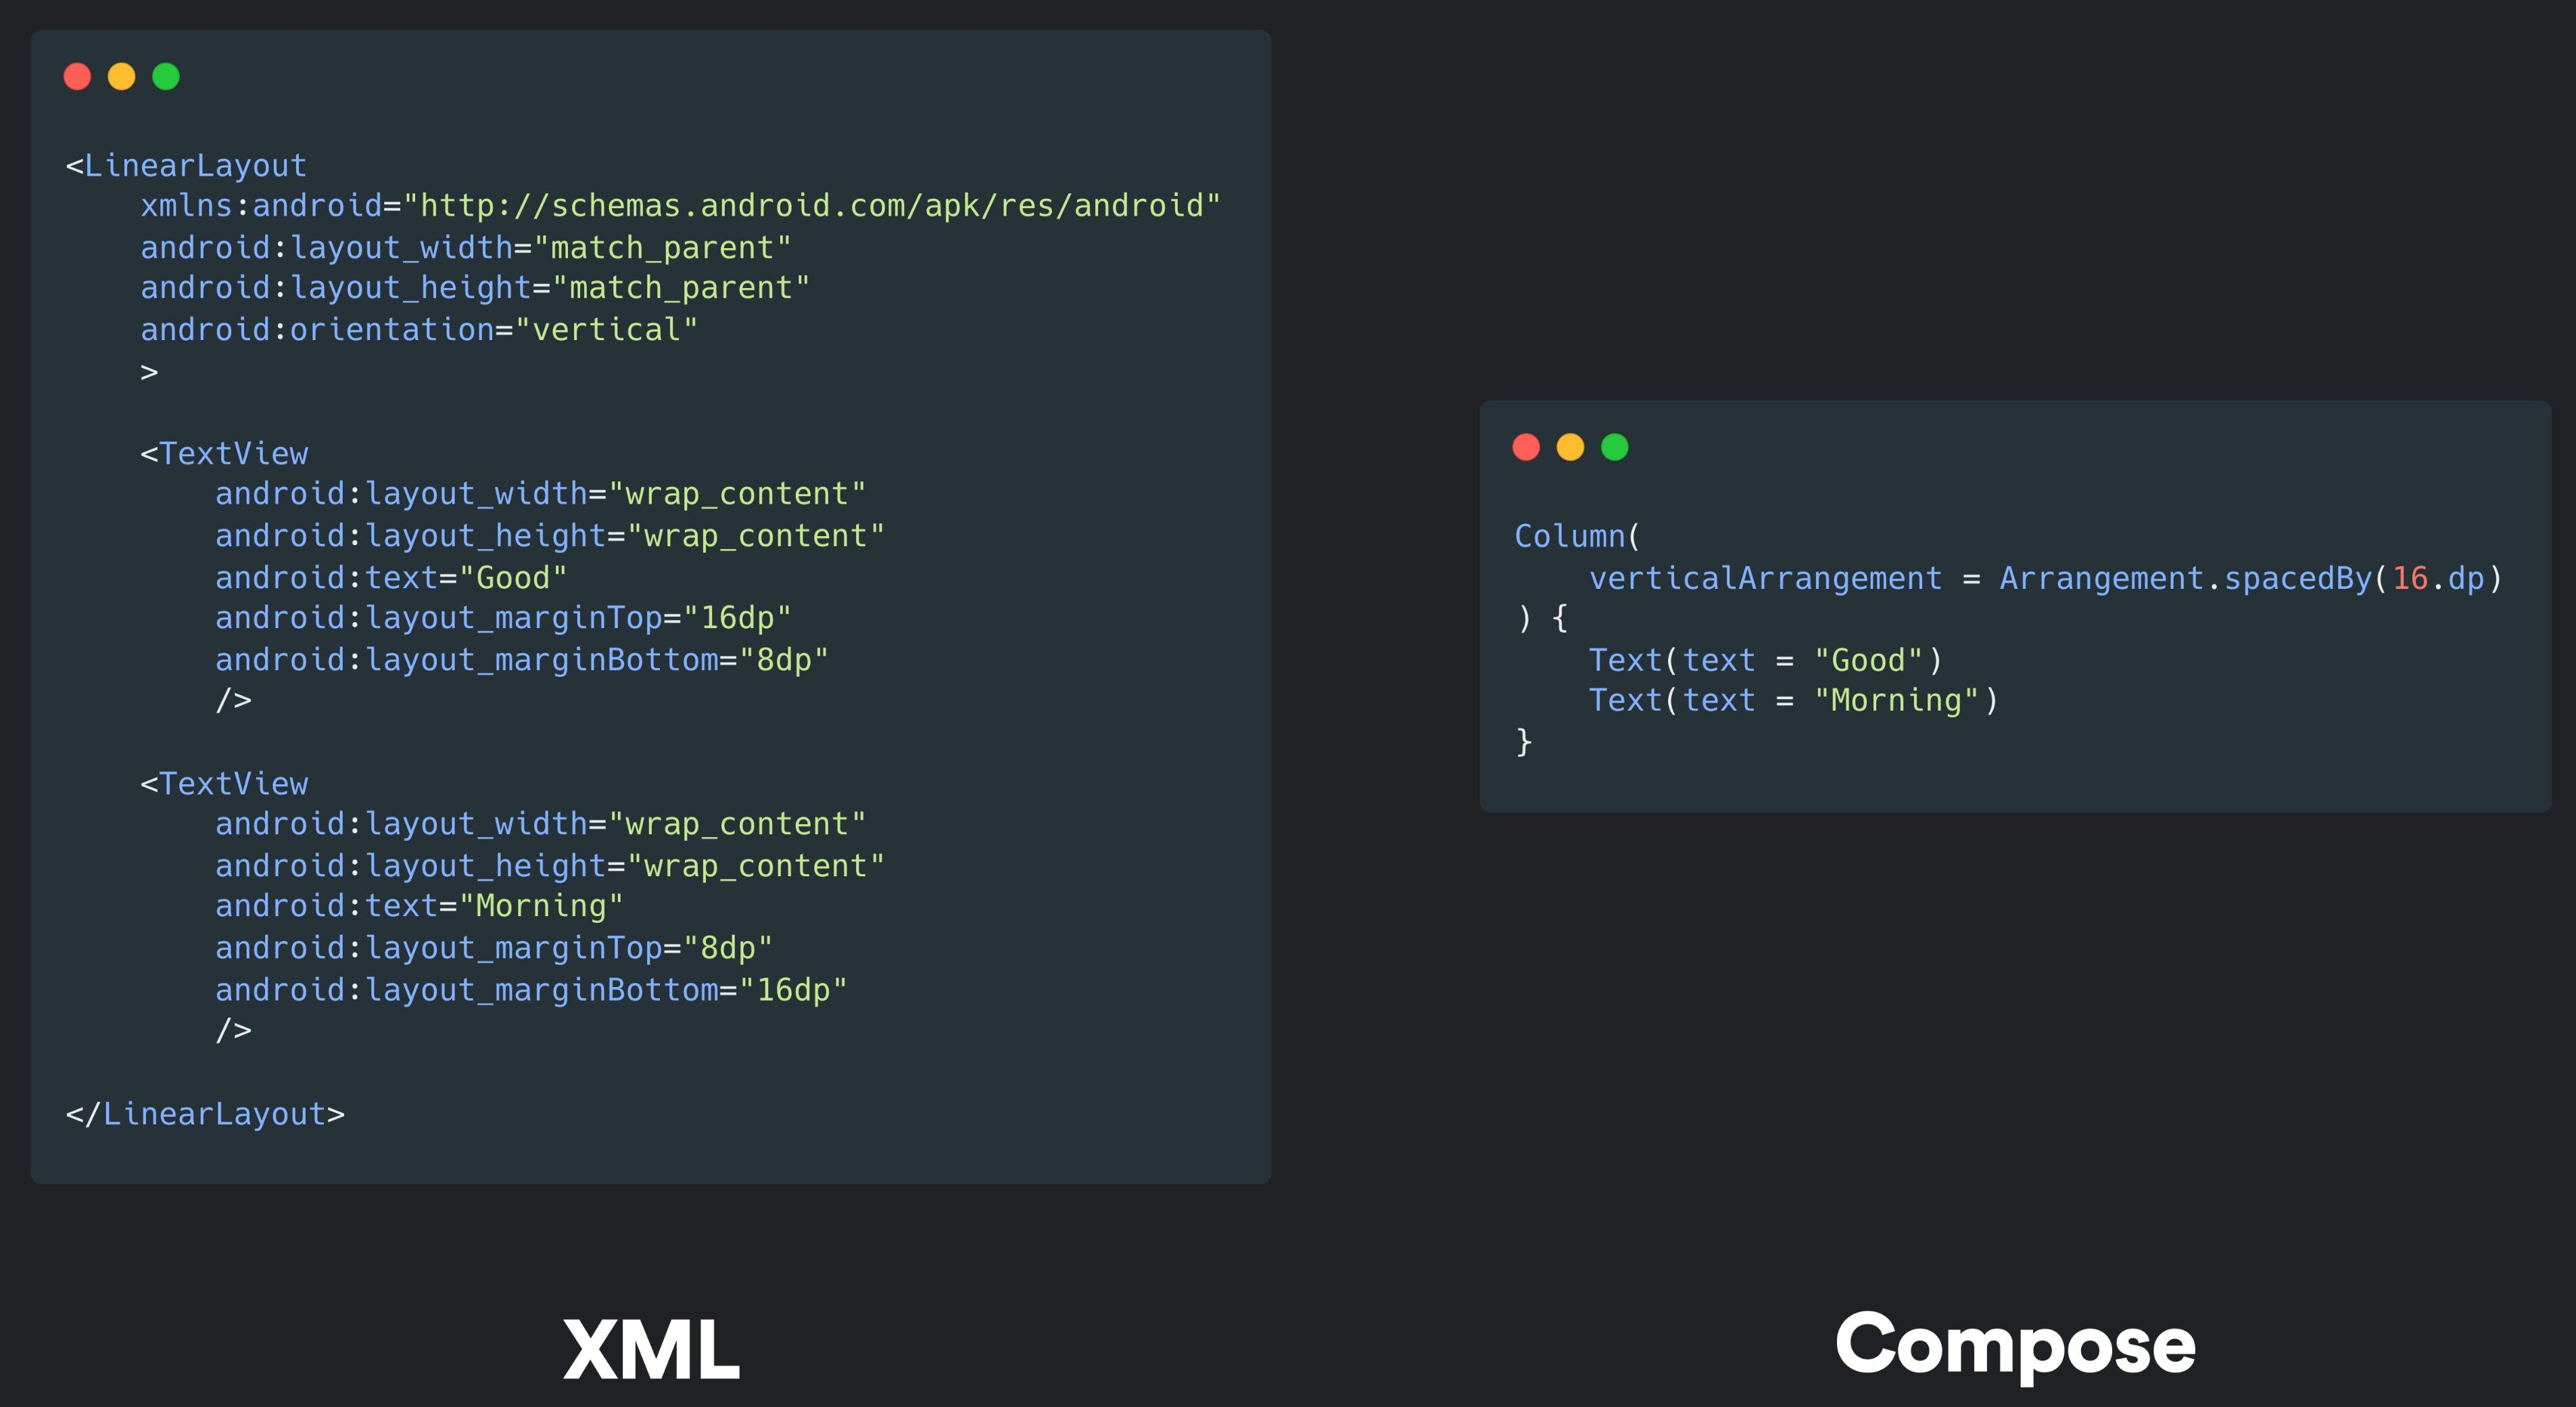
\includegraphics[width=\textwidth]{Figuras/compose_vs_xml.jpg}
\centering
\end{figure}

\pagebreak

La Tabla \ref{tab:comparacion_compose_xml} presenta una comparación detallada entre Jetpack Compose y el sistema tradicional de vistas XML, destacando las ventajas técnicas que justifican la adopción de Compose para el desarrollo del launcher.

\begin{table}[H]
\centering
\caption{Comparación entre Jetpack Compose y vistas XML para desarrollo Android}
\label{tab:comparacion_compose_xml}
\begin{tabular}{|p{0.25\textwidth}|p{0.35\textwidth}|p{0.35\textwidth}|}
\hline
\textbf{Aspecto}{\cellcolor[gray]{0.9}} & \textbf{Jetpack Compose}{\cellcolor[gray]{0.9}} & \textbf{Vistas XML}{\cellcolor[gray]{0.9}} \\
\hline
Paradigma de programación & Declarativo, describe qué mostrar & Imperativo, describe cómo construir \\
\hline
Lenguaje & 100\% Kotlin, fuertemente tipado & XML + Kotlin/Java, tipos débiles \\
\hline
Gestión de estado & Recomposición automática con State & Actualización manual de vistas \\
\hline
Animaciones & APIs nativas integradas, declarativas & Requiere configuración compleja XML/código \\
\hline
Reutilización de código & Composición funcional, alta reutilización & Herencia de vistas, reutilización limitada \\
\hline
Curva de aprendizaje & Requiere conocimiento de programación funcional & Familiar para desarrolladores tradicionales \\
\hline
Rendimiento & Recomposición inteligente, optimizado & Inflado de layouts puede ser costoso \\
\hline
Depuración & Compose Inspector integrado & Layout Inspector tradicional \\ 
\hline
Tamaño de APK & Comparable o menor & Puede ser mayor con layouts complejos \\
\hline
Interoperabilidad & Completa con vistas XML existentes & No compatible con Compose sin wrappers \\
\hline
Soporte de temas & Material Design 3 nativo & Requiere configuración manual extensa \\
\hline
Testing & Testing declarativo con ComposeTestRule & Testing complejo de interacciones UI \\
\hline
Mantenimiento & Simplificado, lógica en un solo lugar & Complejo, lógica distribuida en XML y código \\
\hline
Adopción empresarial & Creciente, recomendado por Google & Establecido, pero en desuso gradual \\
\hline
\end{tabular}
\end{table}

\subsubsection{Persistencia de datos: Room.}

La gestión eficiente de datos constituye un pilar fundamental en DinoLauncher, especialmente considerando las funcionalidades de seguimiento de tareas, hábitos, límites de aplicaciones y configuraciones de usuario que requieren persistencia local. Para satisfacer estos requerimientos, se optó por Room como la solución de base de datos del proyecto, una decisión que se fundamenta tanto en las necesidades específicas del launcher como en las ventajas técnicas que ofrece esta tecnología.

Room es una biblioteca de persistencia desarrollada por Google que forma parte de Android Jetpack, diseñada específicamente para proporcionar una capa de abstracción sobre SQLite. Esta tecnología combina la potencia y flexibilidad de SQLite con la simplicidad y seguridad de tipos que caracteriza al desarrollo moderno en Android. Room facilita significativamente el trabajo con bases de datos locales mediante el uso de anotaciones, eliminando gran parte del código repetitivo tradicionalmente asociado con SQLite.

La implementación de Room en DinoLauncher se evidencia a través de una arquitectura de datos bien estructurada que incluye múltiples entidades como ApplicationsModel, TasksModel, CategoriesModel, HabitsModel, HabitsLogsModel y LimitsModel, todas gestionadas mediante sus correspondientes interfaces DAO y centralizadas en DinoDatabase. Esta estructura permite un manejo eficiente de las relaciones entre entidades, como la relación entre hábitos y categorías, o entre registros de hábitos y hábitos específicos.

Las ventajas principales que motivaron la selección de Room sobre alternativas como Firebase incluyen:

\begin{itemize}
    \item \textbf{Funcionamiento offline completo:} Room garantiza que todas las funcionalidades del launcher operen sin conexión a internet, aspecto crítico para un launcher que debe estar disponible en todo momento independientemente de la conectividad del dispositivo.
    
    \item \textbf{Rendimiento optimizado:} Al almacenar los datos localmente, Room elimina la latencia asociada con las consultas de red, proporcionando respuestas instantáneas para operaciones como la carga de aplicaciones, tareas y hábitos.
    
    \item \textbf{Privacidad y seguridad de datos:} Los datos permanecen completamente en el dispositivo del usuario, eliminando preocupaciones sobre privacidad y cumpliendo con las regulaciones de protección de datos sin requerir configuraciones adicionales.
    
    \item \textbf{Integración nativa con Android:} Room está diseñado específicamente para Android y se integra perfectamente con el ciclo de vida de las actividades y fragmentos, así como con otras bibliotecas de Jetpack como LiveData y ViewModel.
    
    \item \textbf{Verificación en tiempo de compilación:} Room valida las consultas SQL en tiempo de compilación, detectando errores antes de la ejecución y mejorando la estabilidad de la aplicación.
    
    \item \textbf{Soporte completo para corrutinas:} La integración nativa con corrutinas de Kotlin permite operaciones de base de datos asíncronas de manera elegante y eficiente, como se observa en las implementaciones de los casos de uso del proyecto.
    
    \item \textbf{Gestión automática de migraciones:} Room facilita las actualizaciones de esquema de base de datos mediante un sistema de migraciones robusto y controlado.
    
    \item \textbf{Menor complejidad de configuración:} No requiere configuración de servicios externos, autenticación o gestión de conexiones de red, simplificando significativamente el desarrollo y mantenimiento.
\end{itemize}

La Tabla \ref{tab:comparacion_room_firebase} presenta una comparación detallada entre Room y Firebase, destacando los aspectos técnicos y funcionales que justifican la elección de Room para DinoLauncher.

\begin{table}[H]
\centering
\caption{Comparación entre Room y Firebase para DinoLauncher}
\label{tab:comparacion_room_firebase}
\begin{tabular}{|p{0.25\textwidth}|p{0.35\textwidth}|p{0.35\textwidth}|}
\hline
\textbf{Aspecto} & \textbf{Room} & \textbf{Firebase} \\
\hline
Almacenamiento & Local SQLite en el dispositivo & Remoto en la nube de Google \\
\hline
Conectividad & Funciona completamente offline & Requiere conexión a internet \\
\hline
Rendimiento & Acceso instantáneo a datos locales & Latencia por consultas de red \\
\hline
Privacidad & Datos completamente privados & Datos almacenados en servidores externos \\
\hline
Sincronización & No aplicable, datos locales únicamente & Sincronización automática entre dispositivos \\
\hline
Configuración inicial & Mínima, integración directa & Requiere configuración de proyecto en consola \\
\hline
Costos & Gratuito completamente & Gratuito hasta ciertos límites, luego de pago \\
\hline
Escalabilidad & Limitada por almacenamiento del dispositivo & Alta escalabilidad en la nube \\
\hline
Autenticación & No requerida & Sistema de autenticación necesario \\
\hline
Backup automático & No incluido nativamente & Automático en la nube \\
\hline
Consultas complejas & SQL completo disponible & Limitaciones en consultas complejas \\
\hline
Integración Android & Nativa con Jetpack & Buena pero requiere SDKs adicionales \\
\hline
Verificación de tipos & Compilación con verificación SQL & Tipos dinámicos en tiempo de ejecución \\
\hline
Gestión de relaciones & Soporte completo para foreign keys & Requiere desnormalización de datos \\
\hline
Control de versiones & Migraciones controladas localmente & Versionado manejado por Firebase \\
\hline
\end{tabular}
\end{table}

La arquitectura implementada en DinoLauncher demuestra las ventajas prácticas de Room mediante casos de uso especializados como ApplicationsUseCase, TasksUseCase, CategoriesUseCase, HabitsUseCase y LimitsUseCase, que encapsulan la lógica de negocio y proporcionan una interfaz limpia para la interacción con la base de datos. Esta estructura facilita el mantenimiento del código, mejora la testabilidad y asegura la separación de responsabilidades en la aplicación.

La decisión de utilizar Room se alinea perfectamente con la filosofía de DinoLauncher de promover la productividad y minimizar las distracciones, ya que elimina la dependencia de conectividad externa y garantiza un funcionamiento consistente y rápido en todas las circunstancias de uso.
\subsection{Levantamiento de requerimientos.}

Para llevar a cabo el desarrollo del launcher Android enfocado en combatir la procrastinación en estudiantes universitarios, se utilizaron múltiples técnicas de recolección de información que representaran de una manera clara las acciones a realizar para cumplir los objetivos, desde la teoría hasta la manera en cómo se interactúa con los dispositivos móviles. A continuación, se detallan las técnicas empleadas y los resultados obtenidos:

\subsubsection{Metodología empleada.}

\textbf{Lluvia de ideas (Brainstorming):} Se recurrió a la técnica de brainstorming para generar un amplio abanico de ideas sobre las funcionalidades que el launcher podría ofrecer. A través de sesiones creativas, se exploraron diversas posibilidades y se identificaron las características más importantes que podrían contribuir a mejorar la productividad de los estudiantes. Esta técnica permitió establecer el conjunto inicial de funcionalidades como la gestión de tareas, gestión de hábitos y control de tiempo de uso de aplicaciones, en conjunto con sus particularidades a nivel de desarrollo y diseño.

\textbf{Observación:} Al analizar la interacción de los estudiantes con sus dispositivos móviles en entornos académicos, especialmente de la Universidad del Valle en Tuluá, se identificó que muchos de ellos utilizan aplicaciones de mensajería, redes sociales y juegos como una forma de distracción y abren dichas aplicaciones muchas veces por mera memoria muscular. Esta observación llevó a la conclusión de que un launcher que si, a nivel visual, reduce los estímulos que faciliten la detección de dichas aplicaciones, puede contribuir a que sean usadas con menor frecuencia. Es por esto que se definió que la interfaz debía ser minimalista, dejando de lado los íconos que caracterizan a cada aplicación por considerarse un disparador que apunta hacia el inmediato uso de la misma. Este proceso también reafirmó la necesidad de implementar un limite de tiempo a aplicaciones que el usuario identifique que necesita regular.

\textbf{Análisis de documentación:} Se revisaron cuatro artículos relacionados con la procrastinación académica, los cuales sirvieron de apoyo para entender mejor el contexto en el que se desarrollaría el launcher.

Durante el análisis se identificaron patrones de comportamiento que van más allá del simple uso de dispositivos móviles. Los estudios revisados revelaron que existe una relación negativa entre la procrastinación académica y las intenciones de llevar a cabo conductas saludables, asociada con una menor autoeficacia específica de la salud y bajo control conductual percibido. Se encontró evidencia de una correlación directa de intensidad moderada a fuerte entre la postergación de actividades académicas y la dependencia al dispositivo móvil, siendo especialmente notable en estudiantes universitarios donde el 59,3\% presenta niveles moderados de dependencia.

La investigación también demostró que el uso problemático del smartphone va más allá de las aplicaciones de mensajería y redes sociales, extendiéndose a lo que se denomina "procrastinación electrónica", que abarca el uso excesivo de computadoras, videojuegos, televisión, películas y consumo de noticias. Esta forma de procrastinación resulta particularmente seductora debido a la accesibilidad constante que proporciona internet, permitiendo la distracción en cualquier momento del día.

Los hallazgos confirman que a mayor uso problemático del smartphone, mayor es la tendencia a procrastinar en los estudiantes, y dado que este uso parece estar relacionado con un bajo autocontrol, se identificó la necesidad de implementar programas de intervención relacionados con la resiliencia para controlar el uso del smartphone y mejorar la gestión del tiempo. Estos insights fueron fundamentales para definir las funcionalidades del launcher, especialmente las relacionadas con el control de tiempo de uso y el modo concentración.

La combinación de estas técnicas permitió construir una base sólida para el desarrollo del launcher. Los resultados obtenidos a través de este proceso de levantamiento de requerimientos fueron fundamentales para definir los requisitos funcionales y no funcionales del sistema, asegurando así que el producto final respondiera de manera efectiva a las necesidades de los usuarios.

\subsubsection{Requerimientos funcionales.}

Los requerimientos funcionales identificados se organizaron en las siguientes categorías principales:

\begin{enumerate}
    \item \textbf{Lanzador de aplicaciones:} Funcionalidad principal del launcher que mostrará la lista de aplicaciones disponibles para su ejecución. Incluirá gestión básica de aplicaciones mediante pulsación prolongada para desinstalar, acceder a información de la aplicación o fijar aplicaciones en el escritorio.
    
    \item \textbf{Accesos rápidos:} Sistema de accesos directos para aplicaciones esenciales predeterminadas como correo electrónico,cámara o teléfono, sin necesidad de búsqueda. Permitirá la personalización mediante el fijado de aplicaciones al escritorio.
    
    \item \textbf{Búsqueda integrada:} Barra de búsqueda que mostrará aplicaciones que coincidan con el texto ingresado, así como configuraciones específicas del launcher.
    
    \item \textbf{Modo concentración:} Sistema de bloqueo temporal de aplicaciones que impedirá su uso hasta la desactivación manual o automática del modo. Incluirá bloqueo de notificaciones de aplicaciones restringidas y programación automática basada en horarios académicos.
    
    \item \textbf{Control de tiempo de uso:} Funcionalidad para establecer límites de tiempo en aplicaciones específicas. Una vez agotado el tiempo permitido, se implementará un período de espera antes de permitir el uso nuevamente.
    
    \item \textbf{Gestión de tareas:} Sistema tipo to-do que permitirá asignar fechas específicas a las tareas. Las tareas sin fecha asignada aparecerán diariamente hasta su completación. Incluirá sistema de etiquetas para clasificación y organización.
    
    \item \textbf{Gestión de hábitos:} Implementación de tareas recurrentes programadas para días específicos de la semana, con fechas de inicio y fin definidas. Permitirá marcado de completación similar al sistema de tareas.
    
    \item \textbf{Integración Pomodoro:} Herramienta de productividad configurable que permitirá establecer número de sesiones, duración de sesiones de trabajo y tiempos de descanso.
\end{enumerate}

\subsubsection{Requerimientos no funcionales.}

Los requerimientos no funcionales establecidos para el proyecto incluyen:

\begin{itemize}
    \item \textbf{Compatibilidad:} El launcher debe ser compatible exclusivamente con el sistema operativo Android, diseñado específicamente para smartphones (no tablets).
    
    \item \textbf{Rendimiento:} Debe ofrecer un rendimiento óptimo aprovechando las ventajas del desarrollo nativo en Android.
    
    \item \textbf{Usabilidad:} Interfaz minimalista con diseño centrado en el usuario, siguiendo las directrices de Material Design de Android.
    
    \item \textbf{Seguridad:} Implementación de controles de acceso para las funcionalidades de bloqueo y restricción de aplicaciones.
    
    \item \textbf{Mantenibilidad:} Código estructurado y documentado para facilitar futuras actualizaciones y mejoras.
\end{itemize}

\subsubsection{Investigación tecnológica.}

Como parte del proceso de levantamiento de requerimientos, se realizó una investigación exhaustiva para determinar las tecnologías más apropiadas para el desarrollo del launcher.

\textbf{Decisión de desarrollo nativo vs. multiplataforma:}

Se optó por el desarrollo nativo de la aplicación ya que ofrece mejor rendimiento, fácil acceso a todos los recursos del smartphone y está enfocado a un sistema operativo en particular (Android). Los frameworks multiplataforma actuales también ofrecen buen rendimiento e integración con las herramientas de desarrollo de Android, pero son más propensos a tener menor rendimiento, usar más recursos del sistema y generar fallos debido a las diferencias entre iOS y Android.

\begin{table}[H]
\centering
\caption{Comparación desarrollo nativo vs. multiplataforma}
\begin{tabular}{|p{0.25\textwidth}|p{0.35\textwidth}|p{0.35\textwidth}|}
\hline
\textbf{Aspecto} & \textbf{Desarrollo Nativo Android} & \textbf{Desarrollo Multiplataforma} \\
\hline
Lenguaje & Kotlin o Java & JavaScript, Dart, C\# \\
\hline
Rendimiento & Óptimo, optimizado para Android & Bueno, pero inferior debido a abstracción \\
\hline
Acceso a APIs & Total acceso a APIs y hardware & Limitado, requiere plugins específicos \\
\hline
Experiencia UX & Adaptación completa a Material Design & Puede no seguir completamente las directrices \\
\hline
Mantenimiento & Simplificado para Android & Más complejo para compatibilidad específica \\
\hline
\end{tabular}
\end{table}

\textbf{Selección del lenguaje de programación:}

Las dos alternativas de desarrollo nativo en Android son Java y Kotlin. Java es el lenguaje tradicional para el desarrollo Android, pero ha perdido terreno gracias a Kotlin y sus mejoras con respecto a Java para el desarrollo móvil, principalmente en cuanto a sintaxis. Se seleccionó Kotlin por las siguientes razones:

\begin{itemize}
    \item Google recomienda Kotlin para cualquier proyecto nuevo de Android y declaró un enfoque Kotlin-first desde 2019.
    \item Sintaxis más concisa y moderna que reduce el código boilerplate.
    \item Seguridad de tipos nulos que evita NullPointerExceptions.
    \item Totalmente interoperable con Java.
    \item Comunidad activa y gran cantidad de recursos disponibles.
\end{itemize}

\begin{table}[H]
\centering
\caption{Comparación Kotlin vs. Java}
\begin{tabular}{|p{0.25\textwidth}|p{0.35\textwidth}|p{0.35\textwidth}|}
\hline
\textbf{Aspecto} & \textbf{Kotlin} & \textbf{Java} \\
\hline
Sintaxis & Concisa, moderna y legible & Verbosa y tradicional \\
\hline
Seguridad de tipos nulos & Evita NullPointerExceptions & NullPointerExceptions comunes \\
\hline
Compatibilidad Android & Lenguaje oficial recomendado & Compatible pero no recomendado \\
\hline
Características modernas & Coroutines, extension functions, data classes & Introducción más lenta de características \\
\hline
Productividad & Alta debido a sintaxis concisa & Moderada, requiere más código \\
\hline
\end{tabular}
\end{table}

\textbf{Tecnologías complementarias:}

Para el almacenamiento de datos se seleccionó SQLite como base de datos local, considerando su integración nativa con Android y su eficiencia para el manejo de datos de tareas, hábitos y configuraciones del usuario.

\textbf{Versión mínima de Android:}

Considerando que aproximadamente el 70\% de los usuarios poseedores de un smartphone a nivel mundial tienen instalado el sistema operativo Android, se estableció como requisito técnico soportar las versiones de Android más utilizadas para maximizar la compatibilidad y alcance del launcher.
\subsection{Scrumban: Implementación.}

La gestión eficiente del proceso de desarrollo constituye un factor determinante en el éxito de cualquier proyecto de software. Para este launcher, se adoptó el framework \textit{Scrumban}, una metodología híbrida que combina la estructura organizacional de Scrum con la flexibilidad visual de Kanban. Esta elección se fundamenta en la necesidad de mantener un desarrollo ágil y adaptativo, característico de Scrum, mientras se aprovecha la organización y visualización coherente de actividades que proporciona el tablero Kanban.

Scrumban resulta particularmente adecuado para proyectos individuales, donde la flexibilidad para ajustar prioridades y la capacidad de visualizar el flujo de trabajo son más importantes que las ceremonias tradicionales de Scrum.

\subsubsection{Sprints.}

El proceso de desarrollo se estableció en sprints de \textbf{dos (2) semanas} de duración, considerándose un ritmo sostenible que permitió la planificación detallada sin comprometer la flexibilidad del proceso. El cronograma de desarrollo se dividió en dos períodos académicos: la fase inicial comprendió desde el 16 de agosto hasta el 19 de diciembre de 2024, seguida de una pausa académica y la posterior reanudación el 21 de febrero de 2025, concluyendo el 29 de mayo de 2025. En total se ejecutaron \textbf{dieciseis (16) sprints} que abarcaron desde la conceptualización inicial hasta la implementación completa del launcher.

Los primeros sprints se dedicaron al modelado conceptual de la aplicación y la definición de requerimientos funcionales y no funcionales. Posteriormente, se desarrollaron los mockups y prototipos de interfaz con el objetivo de tener una base visual y de experiencia de usuario sólida para la siguiente etapa. Finalmente, los sprints restantes se enfocaron en la implementación del launcher utilizando Android Studio y las tecnologías previamente seleccionadas.

\subsubsection{Gestión de actividades: GitHub Projects.}

GitHub Projects fue seleccionada como plataforma de gestión de actividades debido a que ofrece una integración y comunicación directa con el repositorio de la aplicación alojado en GitHub y es extremadamente sencilla de utilizar y configurar para diferentes metodologías o tipos de proyectos. La configuración implementada en GitHub Projects incluyó la selección de la plantilla Kanban para reflejar el flujo de trabajo deseado. Se establecieron columnas que representan los estados del trabajo: \textbf{Backlog, En progreso, En revisión, Completado y Listo}, como se muestra en la Figura \ref{fig:github_projects_tablero_kanban}.

\begin{figure}[ht]
  \caption{Tablero Kanban de GitHub Projects.}
  \label{fig:github_projects_tablero_kanban}
  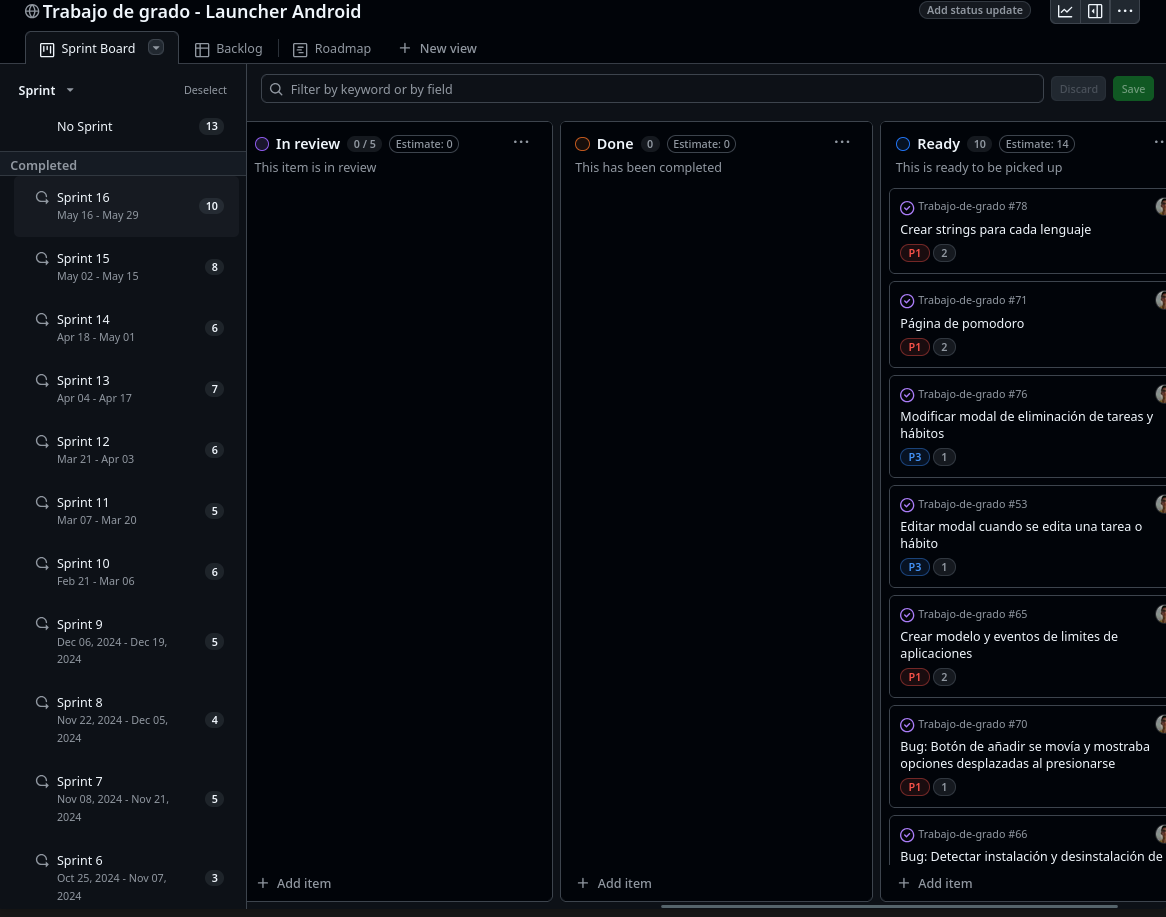
\includegraphics[width=\textwidth]{Figuras/github_projects_tablero_kanban.png}
  \centering
\end{figure}

Las historias de usuario se consignaron en el backlog de GitHub Projects al inicio del proyecto y cada vez que se requería corregir un error o agregar una funcionalidad que no estaba contemplada al inicio del proyecto. Cada historia siguió la estructura estándar de metodologías ágiles: 

\begin{quote}
\centering
\texttt{Como [tipo de usuario],}
\newline
\texttt{quiero [acción]}
\newline
\texttt{para [beneficio].}
\end{quote}

Para historias de mayor complejidad o con aspectos técnicos específicos, se incluyeron criterios de aceptación detallados que establecen las condiciones que deben cumplirse para considerar la funcionalidad como completamente implementada. En la Figura \ref{fig:historia_de_usuario_1}, Figura \ref{fig:historia_de_usuario_2} y Figura \ref{fig:historia_de_usuario_3} se muestran algunos ejemplos de historias de usuario. Para ver la lista completa de historias de usuario, consultar el proyecto en \url{https://github.com/users/Juansebas064/projects/3/views/6}.

\begin{figure}[ht]
  \caption{Ejemplo 1: Historia de usuario.}
  \label{fig:historia_de_usuario_1}
  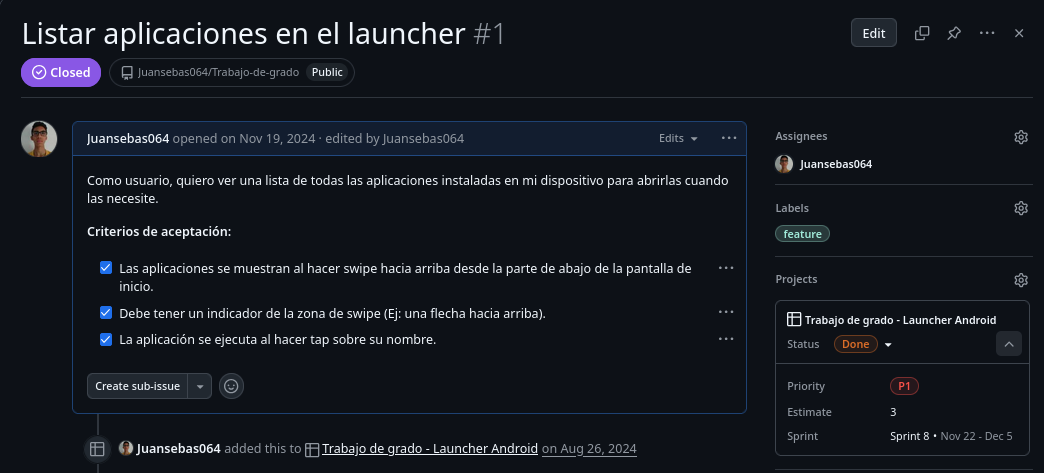
\includegraphics[width=\textwidth]{Figuras/historia_de_usuario_1.png}
  \centering
\end{figure}

\begin{figure}[ht]
  \caption{Ejemplo 2: Historia de usuario.}
  \label{fig:historia_de_usuario_2}
  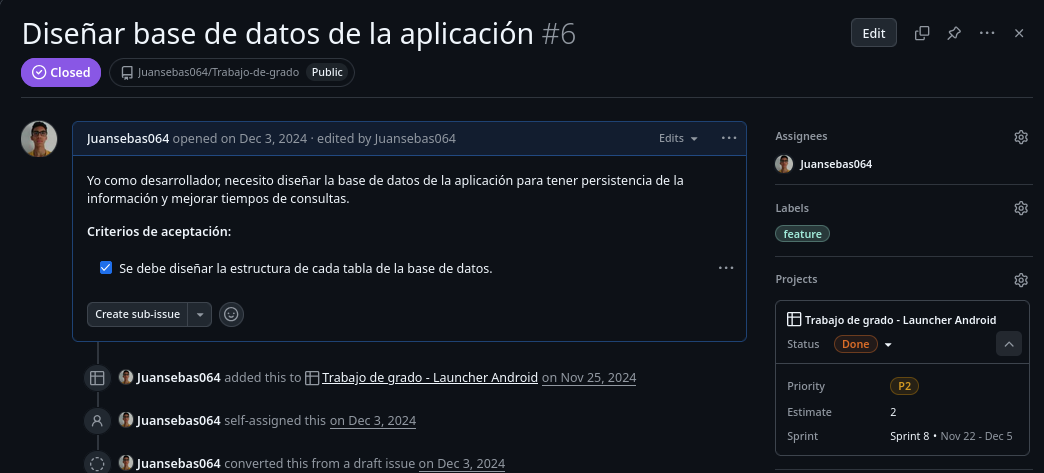
\includegraphics[width=\textwidth]{Figuras/historia_de_usuario_2.png}
  \centering
\end{figure}

\begin{figure}[ht]
  \caption{Ejemplo 3: Historia de usuario.}
  \label{fig:historia_de_usuario_3}
  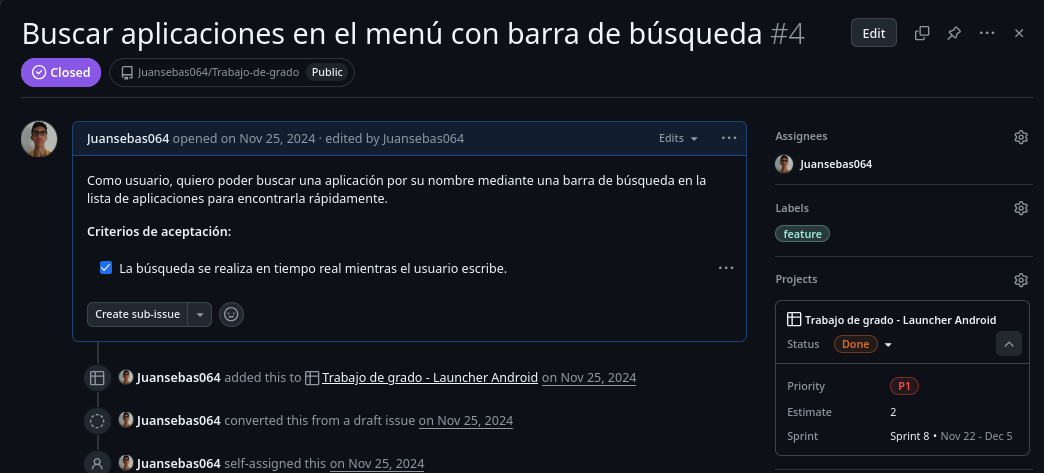
\includegraphics[width=\textwidth]{Figuras/historia_de_usuario_3.png}
  \centering
\end{figure}

\subsubsection{GitHub Flow.}

\textit{GitHub Flow} es una metodología de control de versiones y colaboración en desarrollo de software que se caracteriza por su simplicidad y enfoque en la entrega continua. Desarrollada por GitHub como una alternativa más ágil y menos compleja que \textit{Git Flow}, esta metodología se fundamenta en un flujo de trabajo lineal que prioriza la rapidez de integración y el despliegue frecuente de cambios. La filosofía central de GitHub Flow se basa en mantener la rama principal (main) siempre en un estado desplegable, lo que significa que cualquier código que se integre a esta rama debe estar completamente funcional y listo para producción.

Se buscó que la gestión del proyecto fuera simple pero con una estructura bien definida, este flujo de trabajo se adaptó perfectamente a las necesidades de estandarizar la gestión de ramas de \textit{Git} y de integrar de manera continua los cambios con la rama principal. El proceso de GitHub Flow se estructura en seis pasos: \textbf{Primero}, se crea una nueva rama a partir de la rama principal para cada nueva funcionalidad, corrección de errores o mejora que se desee implementar. Esta rama debe tener un nombre descriptivo (ejemplo: \texttt{apps-limit}) que refleje claramente el propósito del trabajo a realizar.

\textbf{Segundo}, se realizan los commits necesarios en esta rama de trabajo, manteniendo un historial claro y conciso de los cambios implementados.

\textbf{Tercero}, se abre un \textit{Pull Request (PR)} hacia la rama principal, iniciando el proceso de revisión de código. El PR actúa como mecanismo de documentación y discusión sobre los cambios propuestos y protege a la rama principal de ser directamente modificada.

\textbf{Cuarto}, se lleva a cabo la revisión del código en el PR, donde otros miembros del equipo (en el caso de haber varios) evalúan la calidad, funcionalidad y adherencia a los estándares establecidos.

\textbf{Quinto}, una vez que el PR ha sido aprobado y todas las verificaciones automáticas han pasado exitosamente, se procede a la integración del código en la rama principal mediante un \textit{merge}.

\textbf{Sexto}, inmediatamente después de la integración, se procede al despliegue de los cambios en el ambiente de producción, aprovechando que la rama principal se mantiene siempre en estado desplegable (en este caso, la instalación en el dispositivo Android).

En la Figura \ref{fig:ramas_de_github} podemos ver algunas de las ramas que se utilizaron a lo largo del desarrollo del launcher.
\begin{figure}[ht]
  \caption{Gestión de ramas con GitHub Flow.}
  \label{fig:ramas_de_github}
  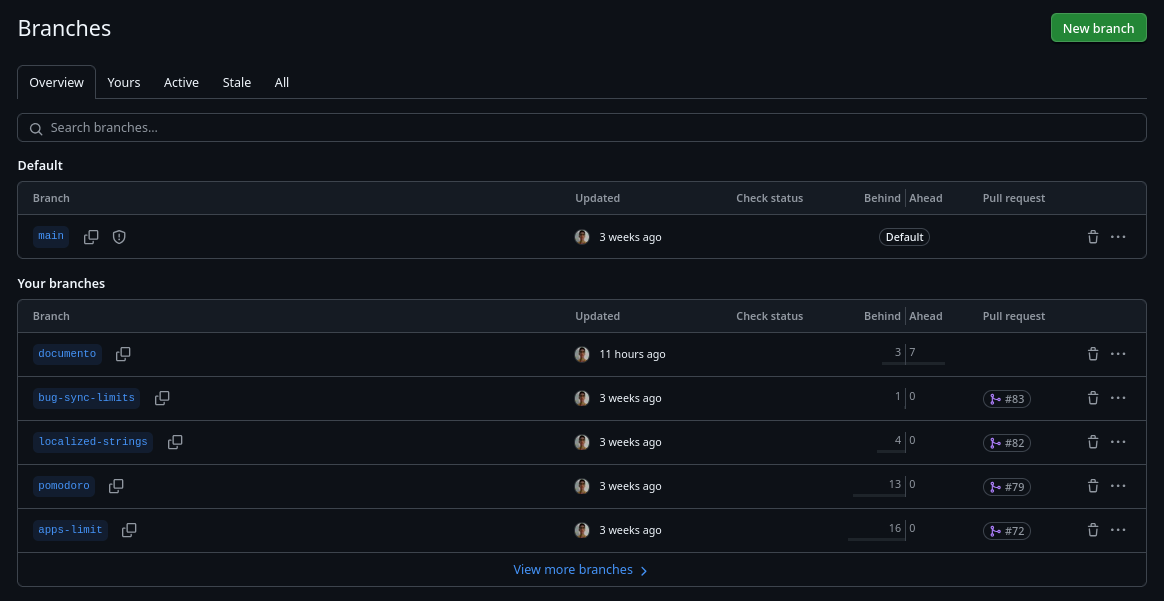
\includegraphics[width=\textwidth]{Figuras/ramas_de_github.png}
  \centering
\end{figure}

%%%%%%%%%%%%%%%%%%%%%%%%%%%%%% Arquitectura y diseño %%%%%%%%%%%%%%%%%%%%%%%%%


\section{Arquitectura y diseño.}

\subsection{Arquitectura.}

\subsubsection{Prácticas recomendadas por Google.}

El desarrollo de aplicaciones Android modernas requiere de una arquitectura clara, modular y escalable, que facilite el mantenimiento del código, la incorporación de nuevas funcionalidades, así como la mejora continua del producto final. Google establece principios fundamentales para el desarrollo de aplicaciones Android robustas y mantenibles a través de la plataforma Android Jetpack \cite{Jetpack}, que han evolucionado a partir de años de experiencia en el ecosistema móvil. Estas prácticas se centran en la separación clara de responsabilidades a través de una \textit{arquitectura basada en capas}, donde cada componente del sistema tiene un propósito específico y bien definido \cite{AndroidBestPractices}. 

La arquitectura recomendada para aplicaciones Android se basa principalmente en tres capas fundamentales:


\begin{itemize}
  \item \textbf{Capa de Presentación (UI):} Encargada exclusivamente de la interacción visual y la experiencia del usuario. Esta capa se ocupa de mostrar la información, escuchar las acciones del usuario y reaccionar a los cambios en el estado de la aplicación. No contiene lógica de negocio ni interacción directa con fuentes de datos, garantizando así una clara separación de responsabilidades.

  \item \textbf{Capa de Dominio (opcional, pero recomendada en proyectos de mediana o gran escala):} Constituye el núcleo lógico del sistema, implementando casos de uso específicos relacionados directamente con las reglas del negocio. Al aislar esta lógica en una capa independiente, se favorece la reutilización de código, la claridad en la implementación y se simplifican significativamente las pruebas unitarias.

  \item \textbf{Capa de Datos:} Responsable de acceder a las fuentes de información, tanto locales como remotas. Utiliza patrones de diseño como el repositorio, el cual se encarga de gestionar una fuente única de verdad para los datos, manteniendo copias locales y actualizando la información desde fuentes externas según sea necesario.
\end{itemize}

Dentro de estas prácticas es especialmente importante destacar el patrón conocido como Flujo Unidireccional de Datos \textit{(Unidirectional Data Flow, UDF)}. En el contexto específico de Android, los datos generalmente fluyen desde elementos con un alcance amplio, como los repositorios y fuentes de datos, hacia elementos con un alcance más limitado, como los componentes visuales de la UI. Por otro lado, los eventos generados por el usuario, como pulsaciones de botones o gestos, fluyen en sentido contrario desde la interfaz gráfica hacia la fuente única de verdad, donde los datos se modifican y actualizan posteriormente, siempre a través de estructuras de datos inmutables.

Este enfoque está estrechamente relacionado con la correcta gestión del ciclo de vida de los componentes Android. El conocimiento explícito y el manejo consciente del ciclo de vida permiten que los componentes reaccionen apropiadamente frente a eventos generados por el propio sistema operativo, como la rotación de pantalla o la suspensión temporal de la aplicación. Herramientas proporcionadas por Android Jetpack, como \textit{ViewModel}, y bibliotecas reactivas como \textit{LiveData} o \textit{Flow}, son clave en este proceso, pues reaccionan de forma automática y segura a los cambios de estado en las actividades y fragmentos.

Google también recomienda emplear bibliotecas especializadas como \textit{Hilt}, para gestionar las dependencias entre componentes. La inyección de dependencias automatiza la creación de objetos en tiempo de compilación sin necesidad de que cada clase los construya. En su lugar, una clase externa se encarga de proveer las dependencias requeridas, lo que simplifica la gestión de dependencias, centraliza las instancias de los objetos y mejora la mantenibilidad del código.


\subsubsection{Patrón de arquitectura MVVM.}

El patrón de arquitectura elegido para el desarrollo del launcher fue \textit{Model-View-ViewModel} (\textit{MVVM}, por sus siglas en inglés), ya que su principal objetivo es separar la lógica de negocio de la interfaz de usuario, obedeciendo a las prácticas recomendadas por Google para el desarrollo de aplicaciones Android \cite{AndroidBestPractices}. Aunque originalmente fue diseñado por Microsoft en 2005 para aplicaciones de escritorio basadas en eventos, con el tiempo ha sido cada vez más implementado en el desarrollo de aplicaciones móviles, especialmente con la introducción de \textit{Android Architecture Components} en la conferencia de Google I/O en 2017 \cite{ArchitectureComponents}. Está inspirado en el patrón \textit{Model-View-Presenter} (\textit{MVP}) y \textit{Model-View-Controller} (\textit{MVC}), manteniendo la separación de responsabilidades e introduciendo un enfoque más reactivo y menos acoplado entre la vista y el modelo. Las principales diferencias entre estos patrones arquitectónicos se presentan en la Tabla \ref{tab:comparacion_arquitecturas}.

\begin{table}[ht]
\centering
\caption{Comparación de patrones arquitectónicos: MVC, MVP y MVVM}
\label{tab:comparacion_arquitecturas}
\begin{tabular}{|p{0.2\textwidth}|p{0.25\textwidth}|p{0.25\textwidth}|p{0.25\textwidth}|}
\hline
\textbf{Aspecto} & \textbf{MVC (Model-View-Controller)} & \textbf{MVP (Model-View-Presenter)} & \textbf{MVVM (Model-View-ViewModel)} \\
\hline
\textbf{Acoplamiento} & View y Model están acoplados. Controller gestiona la interacción. & View y Model están completamente desacoplados por el Presenter. & View y ViewModel están débilmente acoplados a través de enlaces de datos (data binding). \\
\hline
\textbf{Rol de View} & Activa. Puede observar directamente a Model y recibir actualizaciones de Controller. & Pasiva. Implementa una interfaz y no contiene lógica. Presenter indica qué mostrar. & Reactiva. Se enlaza a propiedades de ViewModel y se actualiza automáticamente. \\
\hline
\textbf{Comunicación} & Controller manipula el Modelo. View puede observar al Modelo directamente. & View delega los eventos a Presenter. Presenter actualiza a View a través de una interfaz. & View se suscribe a los flujos de datos de ViewModel. Los eventos de View ejecutan funciones en el ViewModel. \\
\hline
\textbf{Referencia a View} & Controller tiene una referencia directa a View. & Presenter tiene una referencia a View, pero a través de una interfaz abstracta. & ViewModel no tiene ninguna referencia a View. La comunicación es unidireccional (View observa a ViewModel). \\
\hline
\textbf{Testabilidad} & Difícil de probar de forma aislada debido al acoplamiento entre View y Controller. & Alta. Presenter es independiente de la UI de Android y se puede probar fácilmente con mocks. & Muy alta. ViewModel es completamente independiente de View, lo que facilita las pruebas unitarias. \\
\hline
\end{tabular}
\end{table}

El patrón MVVM se compone de tres componentes principales:

\begin{itemize}
  \item \textbf{Model:} Representa la lógica de negocio y los datos de la aplicación. En el launcher, Model incluye las clases que gestionan las tareas, hábitos, límites y preferencias del usuario.

  \item \textbf{View:} Es la interfaz de usuario que muestra los datos al usuario y recibe sus interacciones. Esta capa está implementada utilizando Jetpack Compose.

  \item \textbf{ViewModel:} Actúa como un intermediario entre Model y View. Contiene la lógica para preparar los datos que View necesita y maneja las interacciones del usuario. En el launcher, cada funcionalidad principal (tareas, hábitos, limites y preferencias) tiene su propio ViewModel.
\end{itemize}

\pagebreak

El flujo de datos en MVVM es unidireccional, lo que significa que View observa los cambios en el ViewModel y se actualiza automáticamente cuando los datos cambian. Esto se logra mediante el uso de bibliotecas reactivas como \textit{Flow}, que permite a View suscribirse a los cambios en los datos y reaccionar a ellos sin necesidad de acoplarse directamente a Model. La figura \ref{fig:arquitectura_mvvm} ilustra la relación entre estos componentes.

\begin{figure}[ht]
  \caption{Arquitectura MVVM.}
  \label{fig:arquitectura_mvvm}
  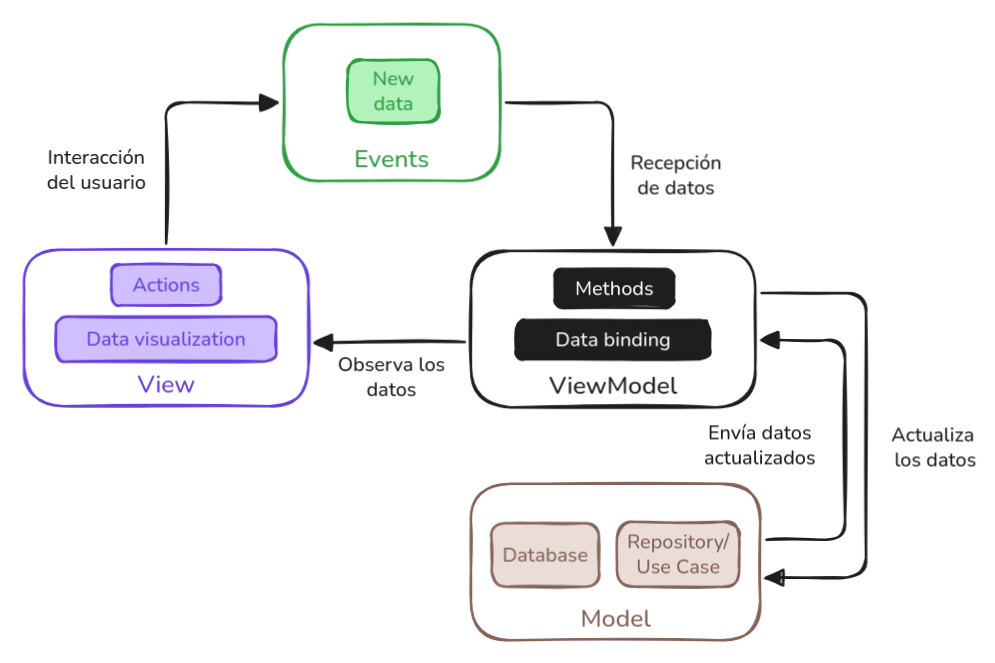
\includegraphics[width=\textwidth]{Figuras/arquitectura_mvvm.png}
  \centering
\end{figure}

\pagebreak

\subsection{Estructura del proyecto.}

La estructura de la aplicación procura seguir cuidadosamente el patrón MVVM y las mejores prácticas de Android, organizando el código en módulos que facilitan el mantenimiento, la escalabilidad y la comprensión del sistema. La organización del proyecto se define de la siguiente manera:

\begin{itemize}
    \item \textbf{config:} Contiene la configuración de la base de datos Room, que centraliza todas las entidades y DAOs del sistema.
    
    \item \textbf{constants:} Almacena las constantes utilizadas a lo largo del proyecto, promoviendo la reutilización de valores y facilitando el mantenimiento del código. Incluye constantes para configuraciones de límites de tiempo, categorías predeterminadas y valores de configuración del sistema.
    
    \item \textbf{data:} Representa la capa de datos del patrón MVVM, implementando el patrón Repository para gestionar el acceso a la información. Esta carpeta encapsula toda la lógica relacionada con la persistencia y recuperación de datos, abstrayendo los detalles de implementación de la base de datos Room.
    
    \item \textbf{di:} Implementa la inyección de dependencias utilizando Dagger-Hilt, siguiendo las recomendaciones de Google para la gestión de dependencias en Android. Esta estructura facilita la creación y provisión automática de instancias de repositorios, casos de uso y ViewModels, mejorando la testabilidad y mantenibilidad del código.
    
    \item \textbf{events:} Define los eventos de la aplicación que facilitan la comunicación entre diferentes componentes del sistema. Implementa un sistema de eventos reactivo que permite la coordinación entre ViewModels y la gestión de estados complejos de la aplicación.
    
    \item \textbf{model:} Contiene las entidades de datos que representan la estructura de información del launcher. Incluye modelos como ApplicationsModel, TasksModel, HabitsModel, CategoriesModel, HabitsLogsModel y LimitsModel, cada uno definiendo la estructura de datos específica para su dominio correspondiente mediante anotaciones de Room.
    
    \item \textbf{navigation:} Gestiona la navegación entre pantallas utilizando Navigation Component de Jetpack, proporcionando una navegación fluida y consistente a través de toda la aplicación. Define las rutas de navegación y maneja las transiciones entre diferentes vistas del launcher.
    
    \item \textbf{services:} Implementa servicios especializados como TimeLimitService para el control de límites de tiempo de aplicaciones y NotificationSender para la gestión de notificaciones del sistema. Estos servicios operan en segundo plano y complementan las funcionalidades principales del launcher.
    
    \item \textbf{states:} Define los estados de la aplicación utilizando clases de datos inmutables que representan el estado de cada pantalla o funcionalidad. Esta estructura facilita la gestión reactiva del estado y la recomposición automática de la interfaz en Jetpack Compose.
    
    \item \textbf{usecases:} Implementa la capa de dominio opcional pero recomendada por Google, encapsulando la lógica de negocio específica de cada funcionalidad. Incluye casos de uso como ApplicationsUseCase, TasksUseCase, HabitsUseCase, CategoriesUseCase y LimitsUseCase, cada uno manejando las operaciones específicas de su dominio respectivo.
    
    \item \textbf{utils:} Proporciona utilidades y funciones auxiliares reutilizables a lo largo del proyecto. Incluye extensiones de Kotlin, formatters de fecha y hora, y otras herramientas que simplifican tareas comunes en la aplicación.
    
    \item \textbf{viewmodel:} Constituye el núcleo del patrón MVVM, implementando los ViewModels específicos para cada funcionalidad principal. Incluye TasksViewModel, HabitsViewModel, LimitsViewModel, PreferencesViewModel y ApplicationsViewModel, cada uno gestionando el estado y la lógica de presentación de su respectiva vista mediante StateFlow y corrutinas de Kotlin.
    
    \item \textbf{views:} Representa la capa de presentación implementada completamente en Jetpack Compose. Esta carpeta se subdivide en módulos específicos que incluyen componentes reutilizables, pantallas principales como TasksAndHabitsListView, MenuView, PreferencesView, y vistas especializadas para la gestión de elementos como ManageTasksHabitsAndCategoriesView. Cada vista observa los cambios en su ViewModel correspondiente y se recompone automáticamente según el estado de la aplicación.
\end{itemize}

Esta estructura modular no solo facilita la implementación del patrón MVVM, sino que también promueve la separación clara de responsabilidades, la reutilización de código y la facilidad de mantenimiento. La organización permite que cada desarrollador pueda ubicar rápidamente los componentes específicos según su función, mientras que la separación entre capas garantiza que los cambios en una parte del sistema no afecten innecesariamente a otras, cumpliendo así con los principios de bajo acoplamiento y alta cohesión recomendados en el desarrollo de software moderno.



%%%%%%%%%%%%%%%%%%%%%%%%%%%%%% Desarrollo %%%%%%%%%%%%%%%%%%%%%%%%%


\section{Desarrollo}
\subsection{Estructura.}

\subsubsection{Proyecto.}

La estructura de la aplicación procura seguir cuidadosamente el patrón MVVM y las mejores prácticas de Android, organizando el código en módulos que facilitan el mantenimiento, la escalabilidad y la comprensión del sistema. La organización del proyecto se define de la siguiente manera:

\begin{itemize}
    \item \textbf{config:} Contiene las configuraciones de la base de datos Room, así como futuros archivos de configuración que pueda necesitar el proyecto.
    
    \item \textbf{di:} Implementa la inyección de dependencias utilizando Dagger-Hilt, siguiendo las recomendaciones de Google para la gestión de dependencias en Android. Hilt facilita la creación y provisión automática de instancias de UseCases y ViewModels.
    
    \item \textbf{events:} Define los eventos de la aplicación que permite la coordinación entre la UI, los ViewModels y la gestión de estados.
    
    \item \textbf{model:} Contiene las entidades de la base de datos que representan la estructura de información del launcher. Incluye modelos para tareas, hábitos, aplicaciones, límites y categorías, cada uno definiendo la estructura de datos específica para su dominio correspondiente mediante anotaciones de Room. Además, incluye clases de estado auxiliares, constantes usadas a lo largo del proyecto y la lógica de negocio encapsulada en UseCases, que representan las operaciones que pueden realizarse sobre los datos, como añadir, eliminar o actualizar tareas y hábitos.
    
    \item \textbf{navigation:} Gestiona la navegación entre pantallas utilizando \textit{Navigation Compose} de Jetpack, proporcionando una navegación fluida y consistente a través de toda la aplicación. Define las rutas de navegación y maneja las transiciones entre diferentes vistas del launcher.
    
    \item \textbf{services:} Implementa servicios especializados para límite de tiempo de aplicaciones, gestión de notificaciones del sistema y actualización de estado de tareas y hábitos al inicio de cada día.
    
    \item \textbf{utils:} Proporciona utilidades y funciones auxiliares reutilizables a lo largo del proyecto.
    
    \item \textbf{view:} Representa la capa de vista implementada completamente en Jetpack Compose. Esta carpeta se subdivide en módulos específicos que incluyen componentes reutilizables, pantallas principales y vistas especializadas para la gestión de elementos. Cada vista observa los cambios en su ViewModel correspondiente y se recompone automáticamente según el estado de la aplicación.
    
    \item \textbf{viewmodel:} Constituye el núcleo del patrón MVVM, implementando los ViewModels específicos para cada funcionalidad principal. Cada ViewModel gestiona el estado y la lógica de presentación de su respectiva vista mediante StateFlow y corrutinas de Kotlin.
\end{itemize}
\subsubsection{Base de datos.}

El modelo de datos del launcher se compone de seis entidades principales, cada una diseñada para encapsular un aspecto específico de la funcionalidad del launcher:

\begin{itemize}
  \item \textbf{ApplicationsModel:} Entidad para gestionar las aplicaciones instaladas en el dispositivo. Esta almacena información esencial sobre cada aplicación que el usuario puede controlar a través del launcher.
  \item \textbf{TasksModel:} Representa las tareas que el usuario puede crear y gestionar dentro del launcher como parte de su sistema de productividad personal.
  \item \textbf{HabitsModel:} Contiene la información relacionada con los hábitos que el usuario desea formar o mantener como parte de su rutina diaria. Esta entidad sigue una estructura similar a las tareas pero está optimizada para el seguimiento a largo plazo.
  \item \textbf{HabitsLogsModel:} Implementa el sistema de seguimiento temporal para los hábitos, permitiendo el registro histórico del cumplimiento de cada hábito a lo largo del tiempo. Esta implementación permite análisis de tendencias y proporciona al usuario retroalimentación sobre su progreso en la formación de hábitos. Aunque fue implementada, no se utilizó en la versión final del launcher, sino que hace parte de trabajos futuros \textbf{REFERENCIA A TRABAJOS FUTUROS}.
  \item \textbf{CategoriesModel:} Este modelo permite al usuario asignar una etiqueta a tareas y hábitos relacionados.
  \item \textbf{LimitsModel:} Gestiona las restricciones de tiempo que el usuario puede establecer para aplicaciones específicas como parte del sistema de control de uso del dispositivo.
\end{itemize}


La relación entre estas entidades y sus atributos se ilustra en la Figura \ref{fig:diagrama_uml}.

\begin{figure}[ht]
  \caption{Diagrama de la base de datos del launcher.}
  \label{fig:diagrama_uml}
  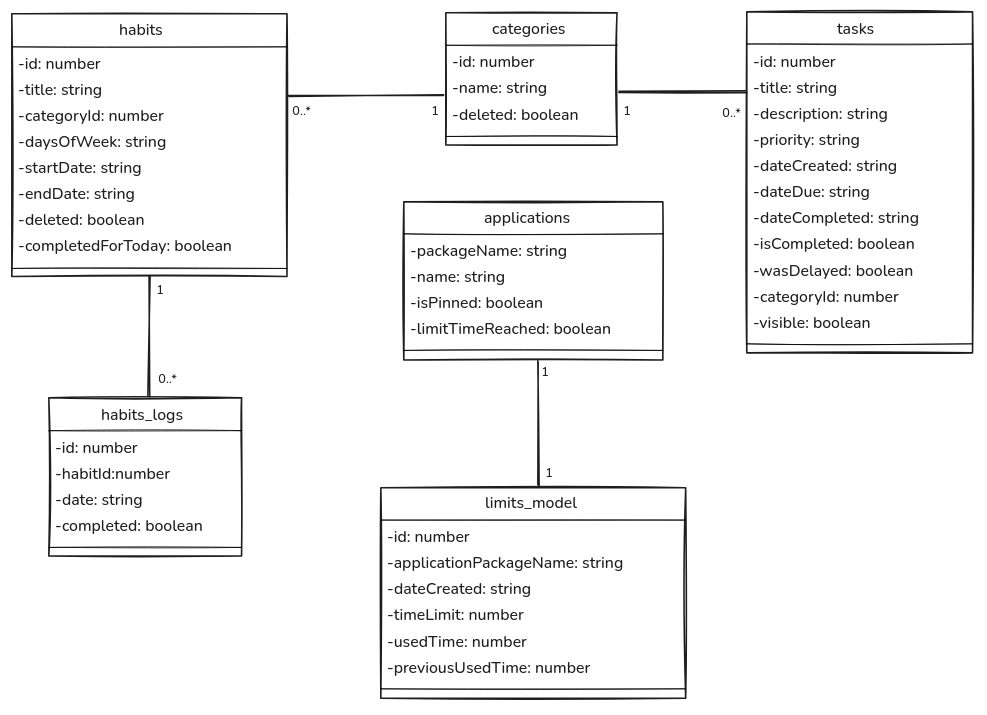
\includegraphics[width=\textwidth]{Figuras/diagrama_uml.png}
  \centering
\end{figure}



%%%%%%%%%%%%%%%%%%%%%%%%%%%%%% Desarrollo %%%%%%%%%%%%%%%%%%%%%%%%%
\section{Pruebas.}
\label{sec:pruebas}

\subsection{Pruebas de usabilidad.}

La evaluación de usabilidad del launcher se realizó mediante una encuesta a estudiantes universitarios, grupo objetivo de la aplicación. Los participantes, jóvenes adultos entre 22 y 25 años que usan su smartphone regularmente, reflejan el perfil típico de usuarios que buscan mejorar su concentración y productividad. La mayoría manifestó ser consciente del tiempo excesivo que pasa en su smartphone, especialmente en momentos inapropiados como durante actividades académicas o de descanso, y expresó interés en herramientas que les ayuden a regular este uso.

Cabe destacar que el número de encuestados fue reducido debido a las particularidades técnicas y éticas del proyecto. Dado que se trata de una aplicación para Android que se debe instalar, no es posible su despliegue en un entorno web ni su distribución pública, ya que su instalación requiere permisos especiales relacionados con acceso a información del sistema operativo y el monitoreo del tiempo de uso de las aplicaciones, aspectos que son sensibles en términos de privacidad.

Por estas razones, se decidió aplicar la encuesta únicamente a un grupo selecto de usuarios que aceptaron instalar la aplicación en sus dispositivos personales y participar bajo las condiciones previamente informadas, garantizando así un entorno de prueba controlado, seguro y éticamente responsable.

La Figura \ref{fig:interfaz_intuitiva} muestra que la mayoría de los participantes considera que el launcher es intuitivo y fácil de usar. El 71,4\% de los participantes calificó con la puntuación máxima (5) la intuición de la interfaz del launcher, mientras que el 28,6\% le otorgó una calificación de 4.

\begin{figure}[h]
  \caption{Primera prueba de usabilidad.}
  \label{fig:interfaz_intuitiva}
  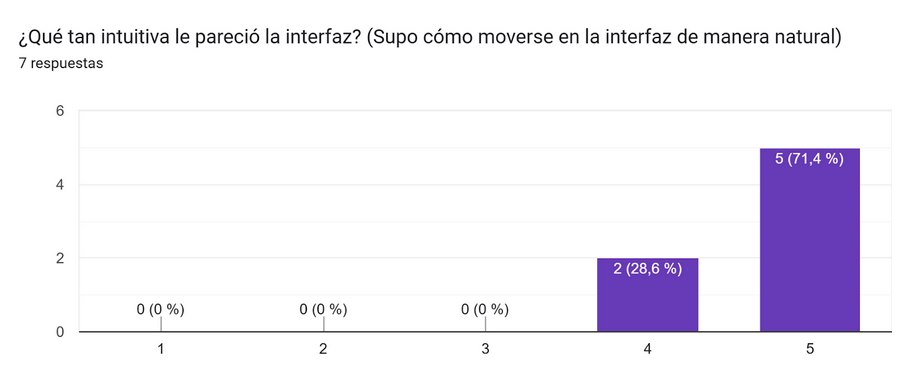
\includegraphics[width=\textwidth]{Figuras/interfaz_intuitiva.png}
  \centering
\end{figure}

En relación con la apariencia de la aplicación, los resultados presentes en la Figura \ref{fig:interfaz_agradable} reflejan una alta aceptación del diseño minimalista, funcional y centrado en la productividad por parte de los usuarios. El 71,4\% de los encuestados calificó el diseño de la interfaz con la puntuación máxima (5), mientras que el 28,6\% otorgó una calificación de 4.

\begin{figure}[h]
  \caption{Segunda prueba de usabilidad.}
  \label{fig:interfaz_agradable}
  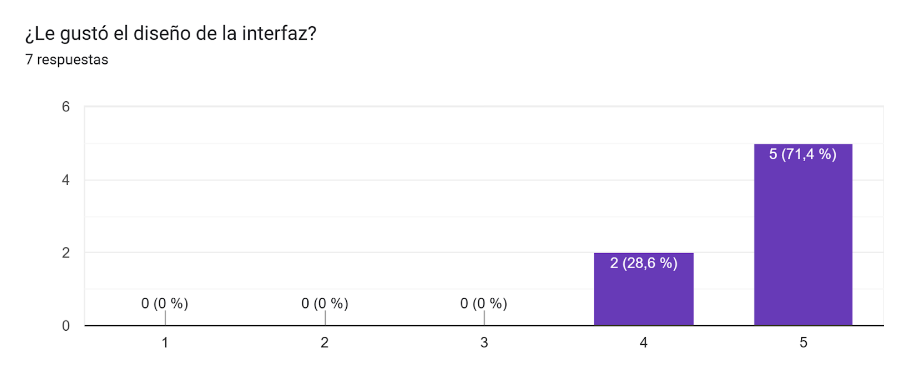
\includegraphics[width=\textwidth]{Figuras/interfaz_agradable.png}
  \centering
\end{figure}

Los resultados de la tercera prueba de usabilidad, mostrados en la Figura \ref{fig:mejores_caracteristicas}, indican que el diseño minimalista fue identificado como la característica más útil del launcher por el 100\% de los participantes. En segundo lugar, se destacan la gestión de tareas y hábitos (71,4\%) y el límite de uso de aplicaciones (71,4\%), dos de las principales funcionalidades del launcher. 

\begin{figure}[h]
  \caption{Tercera prueba de usabilidad.}
  \label{fig:mejores_caracteristicas}
  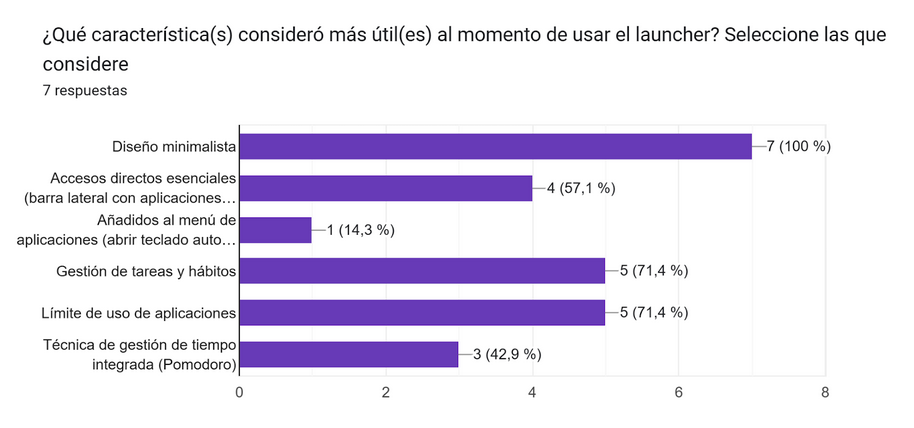
\includegraphics[width=\textwidth]{Figuras/mejores_caracteristicas.png}
  \centering
\end{figure}

El 100\% de los encuestados, según la Figura \ref{fig:cumplio_objetivo}, coincidió en que el launcher cumplió con su objetivo de proporcionar una interfaz de pantalla de inicio minimalista, funcional y con herramientas que pueden ayudar a evitar las distracciones en el uso del Smartphone y ayudar a mejorar la productividad durante el periodo en que fue utilizado.

\begin{figure}[h]
  \caption{Cuarta prueba de usabilidad.}
  \label{fig:cumplio_objetivo}
  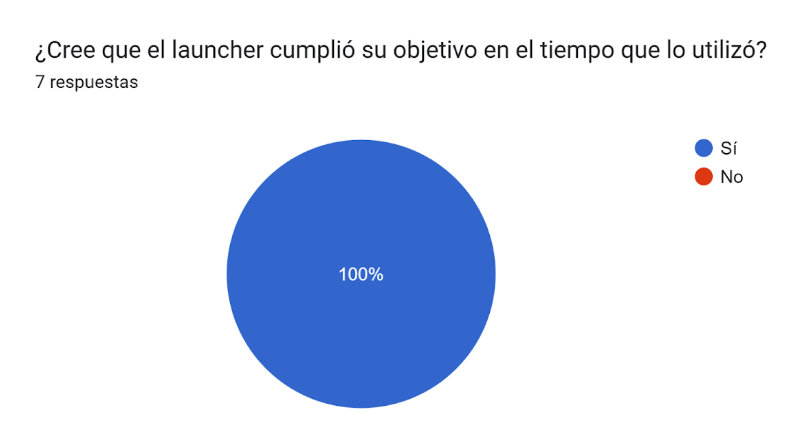
\includegraphics[width=\textwidth]{Figuras/cumplio_objetivo.png}
  \centering
\end{figure}

En respuesta a la pregunta: \textbf{¿Qué fue lo que más le gustó de la aplicación?}, se destacan la funcionalidad de gestión de tareas y hábitos, la practicidad general de la aplicación y su diseño minimalista. También se resaltó el hecho de que las tareas se visualizan de inmediato al iniciar el launcher para mantener el enfoque en las metas personales.

\begin{figure}[h]
  \caption{Quinta prueba de usabilidad.}
  \label{fig:mas_valorado}
  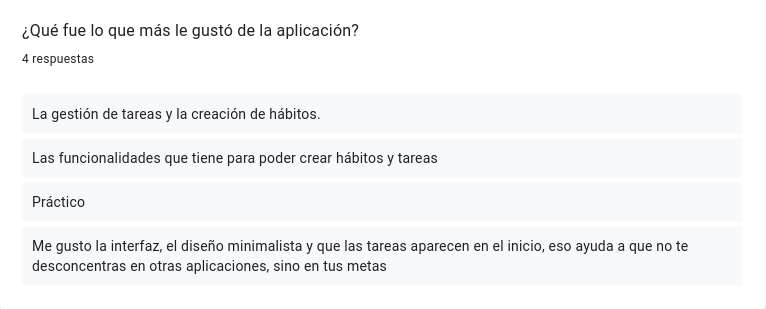
\includegraphics[width=0.92\textwidth]{Figuras/mas_valorado.png}
  \centering
\end{figure}

En cuanto a la pregunta: \textbf{¿Qué fue lo que menos le gustó de la aplicación, qué errores experimentó o en qué podría mejorar?}, los participantes mencionaron principalmente la falta de opciones de personalización, problemas de rendimiento al iniciar la aplicación o al abrir el teclado al entrar al menú de aplicaciones. Por otro lado, uno de los encuestados destacó que la aplicación funcionó sin inconvenientes, lo cual sugiere que la experiencia puede variar según el dispositivo o la configuración.

\begin{figure}[h]
  \caption{Sexta prueba de usabilidad.}
  \label{fig:oportunidades_mejora}
  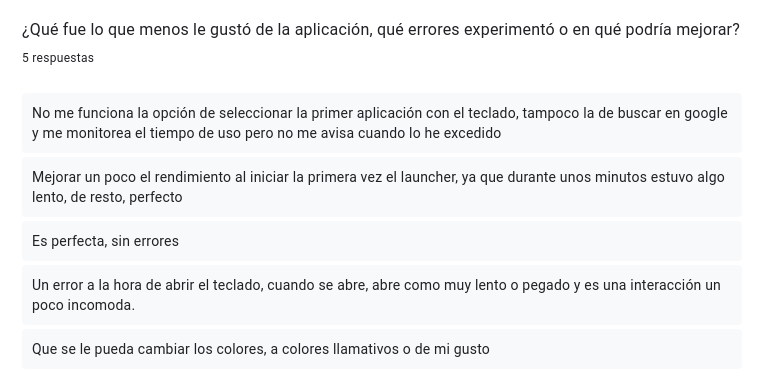
\includegraphics[width=0.92\textwidth]{Figuras/oportunidades_mejora.png}
  \centering
\end{figure}

En respuesta a: \textbf{¿Qué características cree que se podrían añadir que ayuden a cumplir mejor el objetivo de la aplicación?}, los participantes sugirieron una barra de desplazamiento para buscar por orden alfabético las aplicaciones, la posibilidad de bloquear aplicaciones independientemente de si tienen o no límite de tiempo y características de monitoreo de salud, como seguimiento del sueño.

\begin{figure}[h]
  \caption{Séptima prueba de usabilidad.}
  \label{fig:caracteristicas_adicionales}
  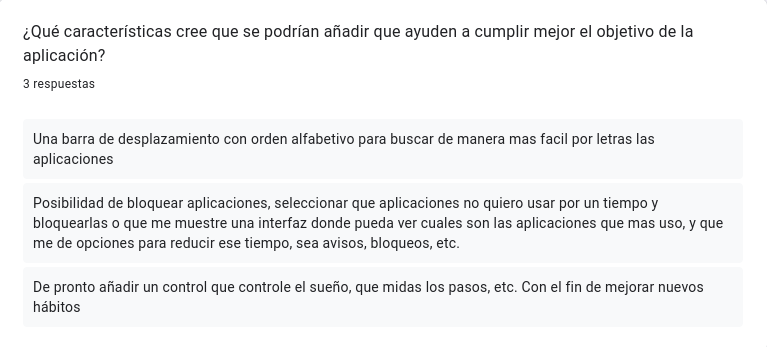
\includegraphics[width=0.92\textwidth]{Figuras/caracteristicas_adicionales.png}
  \centering
\end{figure}

Por último, en la pregunta: \textbf{¿Consideraría seguir usando este Launcher o uno con un enfoque similar en su día a día?}, el 71,4\% de los participantes manifestó su intención de seguir utilizando el launcher o una herramienta con un enfoque similar en su rutina diaria. Por otro lado, el 28,6\% indicó que "tal vez" lo haría, lo cual, aunque no representa una afirmación definitiva, demuestra una disposición positiva hacia la aplicación.

\begin{figure}[h]
  \caption{Octava prueba de usabilidad.}
  \label{fig:continuar_usando}
  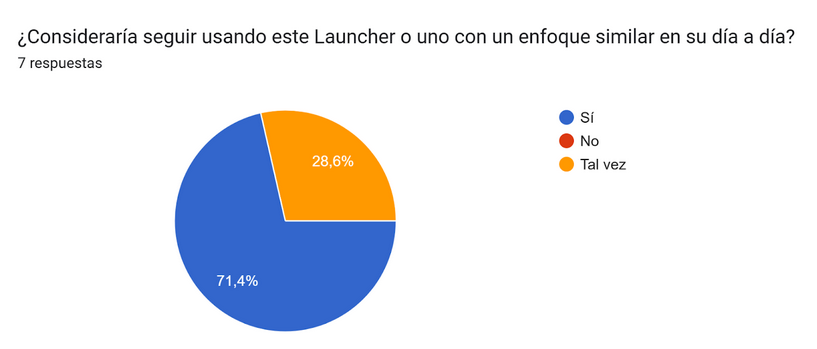
\includegraphics[width=0.92\textwidth]{Figuras/continuar_usando.png}
  \centering
\end{figure}
\subsection{Pruebas unitarias.}

Las pruebas unitarias constituyen un componente fundamental en cualquier proceso de desarrollo de software moderno. Son el primer nivel de pruebas que se realizan para validar la funcionalidad de las unidades más pequeñas del código, como funciones o métodos individuales.

Se desarrollaron pruebas unitarias específicas que cubren los casos de uso que encapsulan la lógica de negocio principal (operaciones con los datos, CRUD). La estrategia de testing adoptada utilizó \texttt{JUnit 4} como framework base y \texttt{mockk} para simluar las entidades usadas en la aplicación real.Los resultados de las pruebas se muestran en la Figura \ref{fig:resultados_pruebas_unitarias}. 

\begin{figure}[ht!]
  \captionof{figure}{Resultados pruebas unitarias.}
  \label{fig:resultados_pruebas_unitarias}
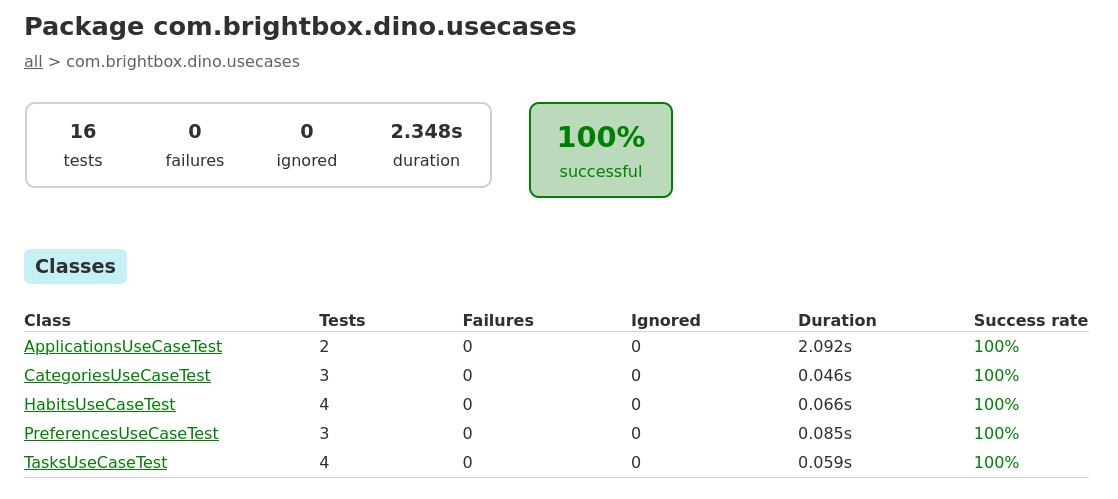
\includegraphics[width=\textwidth]{Figuras/resultados_pruebas_unitarias.png}
  \centering
\end{figure}


%%%%%%%%%%%%%%%%%%%%%%%%%%%%%%Referencias%%%%%%%%%%%%%%%%%%%%%%%%%%%
\bibliography{Bibliografia}


\end{document}
